% ******************************************************************	********************************************
%
% **************************************************************************************************************
\documentclass[ twoside,openright,titlepage,numbers=noenddot,%
								toc=bibliography,toc=listof,%
                footinclude=false,headinclude=false,cleardoublepage=empty,%
								BCOR=5mm,paper=a4,fontsize=11pt,%DIV=14,%
                ngerman%
                ]{scrreprt}

%***************************************************************************************************************
% Note: Make all your adjustments in here
%***************************************************************************************************************
% ****************************************************************************************************
% htwsaar-i-mst-config.tex 
% ****************************************************************************************************  
\RequirePackage[utf8]{inputenc}				
 \DeclareUnicodeCharacter{00A0}{~}								
\RequirePackage[T1]{fontenc} 
								
% ****************************************************************************************************
% 1. Personal data and user ad-hoc commands
% ****************************************************************************************************
\newcommand{\myTitle}{Eine \LaTeX-Vorlage für Abschlussarbeiten im Bereich Informatik/ Mechatronik-Sensortechnik an der htw saar}
\newcommand{\myDegree}{Bachelor of Science (B.\,Sc.)\xspace}
%\newcommand{\myDegree}{Master of Science (M.\,Sc.)\xspace}
\newcommand{\myDegreeType}{Bachelor\xspace}
%\newcommand{\myDegreeType}{Master\xspace}
\newcommand{\myDegreeCourse}{Praktische Informatik}
%\newcommand{\myDegreeCourse}{Kommunikationsinformatik}
\newcommand{\myName}{Max Muster\xspace}
\newcommand{\myUni}{Hochschule für Technik und Wirtschaft des Saarlandes\xspace}
\newcommand{\myCompany}{SoftwareCenter Musterhausen\xspace}
\newcommand{\myFirstProf}{Prof. Dr.-Ing. Andr\'e Miede\xspace}
\newcommand{\mySecondProf}{Prof. Dr. Thomas Kretschmer\xspace}
\newcommand{\myLocation}{Saarbrücken\xspace}
\newcommand{\myTime}{Tag.~Monat~Jahr\xspace}
\newcommand{\currentVersion}{Version 2.1\xspace} % TODO: ggf. über git Versionsinformationen automatisch bereitstellen und verwenden

% ********************************************************************
% Setup, finetuning, and useful commands
% ********************************************************************
\newcounter{dummy} % necessary for correct hyperlinks (to index, bib, etc.)
% ****************************************************************************************************


% ****************************************************************************************************
% 2. Loading some handy packages
% ****************************************************************************************************
% ******************************************************************** 
% Packages with options that might require adjustments
% ******************************************************************** 
\PassOptionsToPackage{ngerman}{babel}   % change this to your language(s)
 \RequirePackage{babel}					
 \RequirePackage{csquotes}
	
\PassOptionsToPackage{language=auto,style=numeric-comp,backend=bibtex8,bibencoding=ascii,maxbibnames=50}{biblatex}
 \RequirePackage{biblatex}	
 \bibliography{Bibliography}			

\PassOptionsToPackage{fleqn}{amsmath}		% math environments and more by the AMS 
 \RequirePackage{amsmath}

% ******************************************************************** 
% Setting up the page and margins
% ******************************************************************** 
\usepackage{geometry}
 \geometry{a4paper,left=25mm,right=35mm,top=25mm,bottom=30mm}
% DIESE WERTE SIND NICHT ZU VERÄNDERN -- DO NOT CHANGE THESE VALUES

% ******************************************************************** 
% General useful packages
% ******************************************************************** 
%\usepackage[automark]{scrpage2}
\PassOptionsToPackage{dvipsnames}{xcolor}
	\RequirePackage{xcolor} % [dvipsnames]  
	\definecolor{ingwi}{cmyk}{.9,0,0,0}
\usepackage{textcomp} % fix warning with missing font shapes
\usepackage{scrhack} % fix warnings when using KOMA with listings package          
\usepackage{xspace} % to get the spacing after macros right  
\usepackage{mparhack} % get marginpar right
%\usepackage{fixltx2e} % fixes some LaTeX stuff <-- ist seit 2015 nicht mehr notwendig
\PassOptionsToPackage{printonlyused}{acronym}
	\usepackage{acronym} % nice macros for handling all acronyms in the thesis
%\renewcommand{\bflabel}[1]{{#1}\hfill} % fix the list of acronyms
\usepackage{booktabs}
\usepackage{multirow}
\usepackage[shadow]{todonotes} %Settings for ToDoNotes
% Eigene Shortcuts fuer laengere Befehle
	\newcommand{\todox}[1]{\todo[inline, size=\small]{#1}}
	%Nummerierte Anmerkungen
	\newcounter{todocounter}
	\renewcommand{\todox}[2][]{\stepcounter{todocounter}\todo[inline, size=\small,caption={\thetodocounter: #2}, #1]{\renewcommand{\baselinestretch}{0.5}\selectfont\thetodocounter: #2\par}}
\usepackage{blindtext}
%\usepackage{footmisc}
% ****************************************************************************************************


% ****************************************************************************************************
% 3. Setup floats: tables, (sub)figures, and captions
% ****************************************************************************************************
\usepackage{tabularx} % better tables
	\setlength{\extrarowheight}{3pt} % increase table row height
%\newcommand{\myfloatalign}{\centering} % to be used with each float for alignment
\usepackage{caption}
\captionsetup{format=hang,font=small}
\usepackage{subfig}
\usepackage{wrapfig}
% ****************************************************************************************************


% ****************************************************************************************************
% 6. Setup code listings
% ****************************************************************************************************
\usepackage{listings} 
%\lstset{emph={trueIndex,root},emphstyle=\color{BlueViolet}}%\underbar} % for special keywords
\lstset{language=[LaTeX]Tex,%C++,
    keywordstyle=\color{RoyalBlue},%\bfseries,
    basicstyle=\small\ttfamily,
    %identifierstyle=\color{NavyBlue},
    commentstyle=\color{Green}\ttfamily,
    stringstyle=\rmfamily,
    numbers=none,%left,%
    numberstyle=\scriptsize,%\tiny
    stepnumber=5,
    numbersep=8pt,
    showstringspaces=false,
    breaklines=true,
    frameround=ftff,
    frame=single,
		texcl=true,
    belowcaptionskip=.75\baselineskip
    %frame=L
} 
%Styles für verschiedene Sprachen festlegen, z.B. Java
\lstdefinestyle{Java}{
belowcaptionskip=1\baselineskip,
  breaklines=true,
  xleftmargin=\parindent,
  language=Java,
	texcl=true,
  showstringspaces=false,
  basicstyle=\footnotesize\ttfamily,
  keywordstyle=\bfseries\color{green!40!black},
  commentstyle=\itshape\color{purple!40!black},
  identifierstyle=\color{blue},
  stringstyle=\color{orange}}
% ****************************************************************************************************    		   


% ****************************************************************************************************
% 6. PDFLaTeX, hyperreferences and citation backreferences
% ****************************************************************************************************
% ********************************************************************
% Using PDFLaTeX
% ********************************************************************
\PassOptionsToPackage{pdftex,hyperfootnotes=false,pdfpagelabels}{hyperref}
	\usepackage{hyperref}  % backref linktocpage pagebackref
\pdfcompresslevel=9
\pdfadjustspacing=1 
\PassOptionsToPackage{pdftex}{graphicx}
	\usepackage{graphicx} 
    

% ********************************************************************
% Hyperreferences
% ********************************************************************
\hypersetup{%
    %draft,	% = no hyperlinking at all (useful in b/w printouts)
    pdfstartpage=1, pdfstartview=Fit,%
		colorlinks=true, linktocpage=true,
		%urlcolor=Black, linkcolor=Black, citecolor=Black, %pagecolor=Black,%
		%urlcolor=brown, linkcolor=RoyalBlue, citecolor=green, %pagecolor=RoyalBlue,%
    % uncomment the following line if you want to have black links (e.g., for printing)
    colorlinks=false, pdfborder={0 0 0},
    breaklinks=true, pdfpagemode=UseNone, pageanchor=true, pdfpagemode=UseOutlines,%
    plainpages=false, bookmarksnumbered, bookmarksopen=true, bookmarksopenlevel=1,%
    hypertexnames=true, pdfhighlight=/O,%nesting=true,%frenchlinks,%
    pdftitle={\myTitle},%
    pdfauthor={\textcopyright\ \myName, \myUni},%
    pdfsubject={},%
    pdfkeywords={},%
    pdfcreator={pdfLaTeX},%
    pdfproducer={LaTeX with hyperref}%
}   

% ********************************************************************
% Setup autoreferences
% ********************************************************************
% There are some issues regarding autorefnames
% http://www.ureader.de/msg/136221647.aspx
% http://www.tex.ac.uk/cgi-bin/texfaq2html?label=latexwords
% you have to redefine the makros for the 
% language you use, e.g., american, ngerman
% (as chosen when loading babel/AtBeginDocument)
% ********************************************************************
\makeatletter
\@ifpackageloaded{babel}%
    {%
       \addto\extrasamerican{%
					\renewcommand*{\figureautorefname}{Figure}%
					\renewcommand*{\tableautorefname}{Table}%
					\renewcommand*{\partautorefname}{Part}%
					\renewcommand*{\chapterautorefname}{Chapter}%
					\renewcommand*{\sectionautorefname}{Section}%
					\renewcommand*{\subsectionautorefname}{Section}%
					\renewcommand*{\subsubsectionautorefname}{Section}% 	
				}%
       \addto\extrasngerman{% 
					\renewcommand*{\chapterautorefname}{Kapitel}%
					\renewcommand*{\sectionautorefname}{Abschnitt}%
					\renewcommand*{\subsectionautorefname}{Abschnitt}%
					\renewcommand*{\subsubsectionautorefname}{Abschnitt}% 
					\renewcommand*{\paragraphautorefname}{Absatz}%
					\renewcommand*{\subparagraphautorefname}{Absatz}%
					\renewcommand*{\footnoteautorefname}{Fu\"snote}%
					\renewcommand*{\FancyVerbLineautorefname}{Zeile}%
					\renewcommand*{\theoremautorefname}{Theorem}%
					\renewcommand*{\appendixautorefname}{Anhang}%
					\renewcommand*{\equationautorefname}{Gleichung}%        
					\renewcommand*{\itemautorefname}{Punkt}%
				}%	
			% Fix to getting autorefs for subfigures right (thanks to Belinda Vogt for changing the definition)
			\providecommand{\subfigureautorefname}{\figureautorefname}%  			
    }{\relax}
\makeatother


% ****************************************************************************************************
% 6. Last calls before the bar closes
% ****************************************************************************************************
% ********************************************************************
% Development Stuff
% ********************************************************************
%\listfiles
\PassOptionsToPackage{l2tabu,orthodox,abort}{nag}
	\usepackage{nag}
%\PassOptionsToPackage{warning, all}{onlyamsmath}
%	\usepackage{onlyamsmath}


% ****************************************************************************************************
% 7. Further adjustments (experimental)
% ****************************************************************************************************
%\usepackage{tocbibind} %Allows us to add Bibliography to ToC
\usepackage{enumitem}
\setdescription{font=\normalfont\bfseries} %Changes the appearance of description items
\usepackage[activate={true,nocompatibility},final,tracking=true,kerning=true,spacing=true,factor=1100,stretch=10,shrink=10]{microtype}


% ********************************************************************
% Using different fonts
% ********************************************************************
%\usepackage{lmodern} % <-- no osf support :-(
%\usepackage[tt=false]{libertine} % [osf]
%\usepackage{luximono} 
\usepackage{mathpazo} 
%\usepackage[urw-garamond]{mathdesign} <-- no osf support :-(

\setkomafont{disposition}{\bfseries}
% ****************************************************************************************************

%********************************************************************
% Hyphenation
%*******************************************************
%\hyphenation{put special hyphenation here}

% ********************************************************************
% GO!GO!GO! MOVE IT!
%*******************************************************
\begin{document}
\frenchspacing
\raggedbottom
\selectlanguage{ngerman} % american ngerman
\pagenumbering{roman}
\pagestyle{plain}
%*******************************************************
% Frontmatter
%*******************************************************
%*******************************************************
% Titlepage
%*******************************************************
\begin{titlepage}\linespread{1.5}\selectfont

\includegraphics[width=\linewidth]{Graphics/htwsaar_Logo_inwi_head_VF_4C_crop}
  \begin{center}
    \large  
    \hfill
    \vfill
    %\begingroup
    %  \Large\bfseries\myDegreeType-Thesis 
    %\endgroup
		
	%	\bigskip
		
    %zur Erlangung des akademischen Grades \\
    %\myDegree \\ 
    %an der \myUni \\
    %im Studiengang \myDegreeCourse \\
    %der Fakultät für Ingenieurwissenschaften \\ 
    
  \vfill
	
  \begingroup
    \Large\bfseries\myTitle 
  \endgroup
	
	\bigskip
	
  vorgelegt von \\
  \myNameOne \\
  \myNameTwo \\
  \myNameThree
	
  \vfill
	
  betreut und begutachtet von \\
  \myFirstProf %\\
  %\mySecondProf 
	
  \vfill
	
  \myLocation, \myTime                   

    \end{center}       
\end{titlepage}   
%\cleardoublepage%*******************************************************
% Declaration
%*******************************************************
\pdfbookmark[0]{Selbständigkeitserklärung}{declaration}
\chapter*{Selbständigkeitserklärung}
%\thispagestyle{empty}

Ich versichere, dass ich die vorliegende Arbeit (bei einer Gruppenarbeit: den entsprechend gekennzeichneten
Anteil der Arbeit) selbständig verfasst und keine anderen als die angegebenen Quellen und
Hilfsmittel benutzt habe.

Ich erkläre hiermit weiterhin, dass die vorgelegte Arbeit zuvor weder von mir noch von einer anderen Person an dieser oder einer
anderen Hochschule eingereicht wurde.

Darüber hinaus ist mir bekannt, dass die Unrichtigkeit dieser Erklärung eine Benotung der 
Arbeit mit der Note \glqq nicht ausreichend\grqq zur Folge hat und einen Ausschluss von der Erbringung 
weiterer Prüfungsleistungen zur Folge haben kann.
\bigskip
 
\noindent\textit{\myLocation, \myTime}

\smallskip

\begin{flushright}
    \begin{tabular}{m{5cm}}
        \\ \hline
        \centering\myName \\
    \end{tabular}
\end{flushright}
%\cleardoublepage%*******************************************************
% Sperrvermerk
%*******************************************************
% Der Sperrvermerk kann entfernt werden, wenn die Arbeit z.B. nicht im 
% Zusammenarbeit mit einem Unternehmen angefertigt wurde oder kein
% Sperrvermerk verlangt wird.

\pdfbookmark[0]{Sperrvermerk}{sperrvermerk}
\chapter*{Sperrvermerk}
%\thispagestyle{empty}

Die vorliegende Arbeit mit dem Titel "`\myTitle"' enthält vertrauliche Daten des Unternehmens \myCompany.

Die Arbeit darf nur dem Erst- und Zweitgutachter sowie befugten Mitgliedern des Prüfungsausschusses zugänglich gemacht werden. 
Eine Veröffentlichung und Vervielfältigung der Arbeit ist -- auch in Auszügen -- nicht gestattet.

Eine Einsichtnahme der Arbeit durch Unbefugte bedarf einer ausdrücklichen Genehmigung des Verfassers und des Unternehmens \myCompany.
 % <-- sollte in der Regel nicht notwendig sein und mit Betreuer/Unternehmen abgeklärt werden
%\cleardoublepage%*******************************************************
% Abstract
%*******************************************************
\pdfbookmark[0]{Zusammenfassung}{Zusammenfassung}
\chapter*{Zusammenfassung}
Kurze Zusammenfassung des Inhaltes in deutscher Sprache, der Umfang beträgt zwischen einer halben und einer ganzen DIN A4-Seite.

Orientieren Sie sich bei der Aufteilung bzw. dem Inhalt Ihrer Zusammenfassung an Kent Becks Artikel: \url{http://plg.uwaterloo.ca/~migod/research/beckOOPSLA.html}.
%\cleardoublepage%*******************************************************
% Acknowledgments
%*******************************************************
\pdfbookmark[0]{Danksagung}{acknowledgments}

% Beispiel für ein sinnvolles Zitat 
\begin{flushright}{\slshape    
    We have seen that computer programming is an art, \\ 
    because it applies accumulated knowledge to the world, \\ 
    because it requires skill and ingenuity, and especially \\
    because it produces objects of beauty.} \\ \medskip
    --- Donald E. Knuth \cite{knuth:1974}
\end{flushright}

\bigskip

\begingroup
	\let\clearpage\relax
	\let\cleardoublepage\relax
	\let\cleardoublepage\relax
	\chapter*{Danksagung}
	Hier können Sie Personen danken, die zum Erfolg der Arbeit beigetragen haben, beispielsweise Ihren Betreuern in der Firma, Ihren Professoren/Dozenten an der htw saar, Freunden, Familie usw.




\endgroup


\cleardoublepage%*******************************************************
% Table of Contents
%*******************************************************
\setcounter{tocdepth}{2} % <-- 2 includes up to subsections in the ToC
\setcounter{secnumdepth}{4} % <-- 3 numbers up to subsubsections

\pdfbookmark[0]{\contentsname}{toc}
\tableofcontents 

% Die weiteren Verzeichnisse folgen am Ende des Dokuments 

                  


%*******************************************************
% Mainmatter
%*******************************************************
\cleardoublepage
\pagenumbering{arabic}
\pagestyle{headings}
%\pagestyle{scrheadings}
%\cleardoublepage%=========================================
% 	   Einleitung     		 =
%=========================================
\chapter{Einleitung}

\section{\LaTeX\ installieren und einrichten}
\subsection{Unter Windows}

Als LaTeX-Distribution unter Windows steht \href{http://www.miktex.org/}{\textit{MikTeX}} zu Verfügung, die als freie Software im Internet erhältlich ist. 
\textit{MikTeX} unterstützt Windows XP, Vista und Windows 7. Neben \textit{MikTeX} wird noch ein PostScript-Interpreter benötigt, 
z.B. GhostScript, zu finden auf \href{http://www.chip.de}{Chip.de}.

\textit{Wichtig:} Bei \textit{MikTeX} unbedingt Vollinstallation auswählen, sonst sind eventuell benötigte Packages nicht vorhanden.
  
\subsection{Unter Linux}

Unter Linux existiert die LaTeX-Distribution \textit{texlive}, die als aktuelle Version aus den Paketquellen geladen werden kann (unter Ubuntu mit 
\lstinline{apt-get install texlive-full}). Auch hier ist ganz wichtig, die volle Distribution zu laden, damit alle Packages zur Verfügung stehen.

\section{Entwicklungsumgebungen}

Hat man die passende Distribution installiert, bieten sich vielerlei Möglichkeiten an ein LaTeX-Projekt anzugehen oder einzelne Dokumente zu editieren. Unter
Windows könnten dies folgende sein:

\begin{description}
 \item [TeXnicCenter] Umfangreiche Entwicklungsumgebung mit Projektorganisation und Autovervollständigung
 \item [TeXLipse] Eclipse-Plugin, das alle Vorteile der Eclipseumgebung mit LaTeX verbindet
 \item [TeXmaker] Einfacher LaTeX-Editor mit Pdf-Direktvorschau
\end{description}


Unter Linux stehen bereit:

\begin{description}
 \item [Gummi] Ebenfalls einfacher LaTeX-Editor mit Direktvorschau
 \item [TeXLipse] Auch für Linux erhältlich
 \item [Kile] Umfangreiche Entwicklungsumgebung, ähnlich wie TeXnicCenter
\end{description}

Nach der Installation muss die Entwicklungsumgebung eingerichtet werden; dazu finden sich viele Anleitungen im Internet, die genau erklären, welche Distribution
auf welche Weise eingerichtet wird. Insbesondere sollte der PDF-Viewer festgelegt werden, damit bei Gummi und TeXmaker die Direktvorschau funktioniert. Manchmal kommt es vor, dass die Ausgabe 
nach dem Kompilieren Umlaute und Sonderzeichen nicht richtig darstellt. Unter Linux hängt dies mit den unterschiedlichen Zeichensätzen zusammen, die unterstützt
werden. Um diese Vorlage zu verwenden ist es notwendig, den verwendeten Zeichensatz des Editors bzw. der Entwicklungsumgebung auf den in diesem Dokument
verwendeten Zeichensatz umzustellen: UTF-8 ohne BOM (Byte Order Mark).

\section{Werkzeuge}
\label{sec:Werkzeuge}

\begin{description}
 \item [\href{http://jabref.sourceforge.net/}{JabRef}] Ein Literaturverwaltungsprogramm, welches das \textit{BibTeX}-Format einsetzt
 und mithilfe einer graphischen Oberfläche das Anlegen von Literaturverzeichnissen vereinfacht.
 
\end{description}

\section{Struktur und Gebrauch der Vorlage}

Die vorliegende Vorlage für Abschlussarbeiten besteht aus einer internen Struktur, die grundsätzlich nicht verändert werden sollte. % Außer, der Student weiß genau, was er tut.

\subsection{Struktur der Vorlage}
\label{subsec:strukturvorlage}

%\begin{figure}
    %\centering
    %\includegraphics[width=0.85\textwidth]{Examples/strukturvorlage}
    %\caption{Verzeichnisbaum der Vorlage}
   %\label{fig:strukturvorlage}
  %\end{figure}


\begin{description}
 \item [htw-i-mst-config.tex] Enthält alle zu ladenden Packages, Styleparameter für Hyperlinks, Codelistings und Literaturverzeichnis sowie globale Parameter 
 für Tabellen und Beschriftungen. Im Besonderen befinden sich hier die Variablen für den eigenen Namen, Titel, Datum der Arbeit, den betreuenden Professor etc.
 
 \item [htw-i-mst-vorlage.tex] Dies ist die Hauptdatei, in der alle notwendigen \textit{*.tex}-Dateien eingebunden werden, die zu dem Dokument gehören. Es empfiehlt sich
 die interne Struktur \textit{nicht} zu verändern. Eigene Kapitel werden an der dafür markierten Stelle eingebunden.
     
 \item [Bibliography.bib] Zentrale Datei für die Literaturangaben, welche man z.B. mit JabRef verwalten kann. 

 \item [Chapters/] Ablageort für alle selbst angelegten Kapitel der Arbeit. Die Aufteilung in eigene Dateien erleichtert die Übersicht über den Quellcode. 
 
 \item [Graphics/] Ablageort für alle im Dokument benötigten Grafikdateien. Gerne darf man hier Unterverzeichnisse zur besseren Strukturierung anlegen.
 
 \item [Examples/] Dieser Ordner enthält die in dieser Vorlage beigefügten LaTeX-Beispiele, welche vor der Abgabe der Arbeit selbstverständlich gelöscht werden sollten.
 
 \item [Frontbackmatter/]
 In diesem Ordner sind all jene Dateien abgelegt, die -- außer dem Kerntext in \textit{Chapters/} -- die Gesamtheit der Abschlussarbeit ausmachen.
      \begin{description}
       \item [Titlepage.tex] Definiert die Titelseite der Abschlussarbeit. Diese Datei muss normalerweise nicht verändert werden.
       \item [Abbreviations.tex] Hier werden alle Abkürzungen hinterlegt, die im Dokument verwendet werden.
       \item [Abstract.tex] Eine kurze Zusammenfassung der Abschlussarbeit wird in diese Datei eingefügt.
       \item [Acknowledgements.tex] Dort finden Danksagungen ihren Platz.
       \item [ConfidentialityClause.tex] Beinhaltet den Sperrvermerk und ist nur zu verwenden, falls dies beispielsweise vom beteiligten Unternehmen gefordert wird.
       \item [Contents.tex] Enthält wichtige Eintragungen in die \textit{Table-of-Contents}. Diese Datei muss normalerweise nicht geändert werden.
       \item [Declaration.tex] Enthält die Selbständigkeitserklärung. Diese Datei darf nicht geändert werden.
       \item [Colophon.tex] Enthält einen Hinweis auf die Urheber dieser Vorlage. Diese Datei darf nicht geändert werden.
       \item [ListOfs.tex] Enthält die Einträge für die Tabellen- und Abbildungsverzeichnisse etc. und muss gewöhnlich nicht verändert werden.
      \end{description}

\end{description}


\subsection{Gebrauch der Vorlage}

Grundsätzlich ist nicht viel zu tun, um die Vorlage für Abschlussarbeiten zu verwenden. Man entpackt den Hauptordner in das gewünschte Verzeichnis und nutzt die Dateien so, wie in
\autoref{subsec:strukturvorlage} beschrieben. Danach werden \textit{alle} Dateien gespeichert und die Hauptdatei, \textit{htwsaar-i-mst-vorlage.tex}, mehrfach kompiliert
(LaTeX benötigt mehrere Durchgänge um z.B. Referenzen richtig zuzuordnen).
Hat man Änderungen in \textit{Bibliography.bib} bzw. \textit{Bibliography.tex} vorgenommen oder neue Zitate z.B. mittels \lstinline{\cite} eingefügt, muss erst mit 
\textit{BibLaTeX} und anschließend mitdem entsprechenden LaTeX-nach-PDF-Compiler übersetzt werden.


	 	% Diese Einbindungen werden natürlich entfernt, wenn es an die richtige
%\cleardoublepage%*****************************************
\chapter{Beispiele}\label{ch:examples}
%*****************************************

%************************************************
%*  Abkürzungen *********************************
%************************************************

\section{Abkürzungen}

Um Abkürzungen zu verwenden, muss über \lstinline|\usepackage{acronym}| das benötigte Package geladen werden. Danach kann man lange Begriffe ganz bequem abkürzen:

So muss man nicht ständig \ac{WLAN} ausschreiben, auch \ac{TCP} lässt sich abkürzen. Würde man im Text \acs{WLAN} oft verwenden, kann man sie, wie hier, nur als
Abkürzung anzeigen lassen - oder bei Bedarf die Erklärung mitliefern (\acf{WLAN}). Weiteres Beispiel könnte die \ac{GoF} sein.

Weitere Informationen sind im \href{http://www.ctan.org/tex-archive/macros/latex/contrib/acronym}{Acronym-Manual} zu finden.
%*********************************************
%*	Biblatex-Beispiel
%*********************************************
\section{Beispiel für BibLaTeX}

BibLaTeX ist ein Package, das einem die Arbeit mit Zitaten bzw. Quellenangaben erleichtern kann. Mit JabRef (\autoref{sec:Werkzeuge}) ist es möglich
\textit{*.bib}-Dateien zu erstellen, in denen alle Angaben zu Autor, Buchtitel, Erscheinungsdatum usw. hinterlegt werden, welche zum passenden Zeitpunkt
abgerufen werden können. Das Literaturverzeichnis wird mittels \lstinline{\printbibliography} ausgegeben.

Im Allgemeinen wird im Literaturverzeichnis auch nur jene Literatur aufgenommen, die auch in der \textit{*.tex}-Datei referenziert wird. Danach ist es wichtig
nicht nur mit \textit{Pdf\-LaTeX}, sondern auch mit \textit{BibLaTeX} zu kompilieren, damit die zitierten Einträge in die verschiedenen Hilfsdateien aufgenommen
werden können. %Hinweis: Pdf\-LaTeX teilt LaTeX mit, dass nur zwischen Pdf und LaTeX getrennt werden darf


\subsection*{Einige Zitate}
In diesem Satz könnten wir auf \cite{knuth:1976} verweisen, ebenso auf das wichtige Werk \cite{dueck:trio}. Wenn uns das nicht genug ist, sollten wir das anmerken,
was in \cite{sommerville:1992} geschrieben wurde. Im Zweifelsfall verweisen wir auf eine einzelne Seite, wie in \cite[112]{bentley:1999} zu finden. 

Üblicherweise wird auch der Name des Autors bzw. der Autoren genannt, also beispielsweise bei einem Verweis auf \citeauthor{knuth:1976} \cite{knuth:1976} oder 
auch bei mehreren Autoren \citeauthor{cormen:2001} \cite{cormen:2001}. LaTeX stellt Mechanismen zur Verfügung, auch dies automatisiert zu erledigen.





\section{Referenzierungen}
Mit Referenzierungen kann ich ganz bequem auf Textpassagen, Kapitel, Sections oder Abbildungen im weiteren Text verweisen.
Dies ist ein Verweis auf \autoref{subsec:Beispieltext}, der sich auf \autoref{subsec:Beispieltext} befindet.

Auch ein Verweis auf \autoref{tab:beispieltabelle1} auf Seite~\pageref{tab:beispieltabelle1} ist möglich.

Man sollte beachten, dass man sein Dokument, wenn es Referenzierungen enthält, mehrmals kompiliert, da sonst manche
Verweise nicht aufgelöst werden können.


\subsection{Beispieltext}\label{subsec:Beispieltext}
\blindtext

\section{Dateien einbinden}

Damit man nicht alle Einstellungen, Optionen, Packages und Texte, Abbildungen etc. in einer Datei unterbringen muss, werden
zwei Befehle bereitgestellt, um externe \textit{*.tex}-Dateien einzubinden: \lstinline|\include{PFAD}| und \lstinline|\input{PFAD}|.
Mit dem erstem Befehl wird eine neue Seite angelegt, danach kommen die Inhalte aus der angegebenen Datei; mit dem zweiten
Befehl wird keine neue Seite angelegt -- der Inhalt der angegebenen Datei wird direkt an die betroffene Stelle eingefügt.

\textbf{Wichtig:} Der \textit{Pfad} wird sinnigerweise \textit{relativ} angegeben, wobei als Stammverzeichnis jenes Verzeichnis
angesehen wird, in dem die \textit{*.tex}-Datei mit der \textit{Document}-Umgebung abgelegt ist (in diesem Fall ist es 
\textit{htwsaar-i-mst-config.tex}).
%************************
%*		Tabellen 		*
%************************

\section{Tabellen}
\label{sec:Tabellen}

\subsection{Einfache Tabelle}
In LaTeX lassen sich Tabellen unterschiedlicher Ausprägung einfach erzeugen. Das allgemeine Format einer Tabelle sieht aus wie folgt:

\begin{lstlisting}[caption={Allgemeines Format}]
\begin{table}
	\caption{BESCHRIFTUNG}
	\begin{tabular}{FORMATIERUNG}
		TABELLENINHALT
	\end{tabular}
\end{table}
\end{lstlisting}

Eine Beispieltabelle (Tabelle \ref{tab:beispieltabelle1}) könnte also so aussehen:

\begin{lstlisting}[caption={Tabelle \ref{tab:beispieltabelle1}}]
\begin{table}
	\caption{Beispiel 1}
	\begin{tabular}{lrcr}
		\toprule
		\textbf{Name} & \textbf{Vorname} & \textbf{Matrikelnummer} & \textbf{Lieblingsspeise}\\
		\midrule
		Jackson & Michael & 123456 & Erdbeereis \\
		Springsteen & Bruce & 234567 & Schwedisches Lakritz \\
		Bach & Anna, Magdalena & 3456789 & Frankfurter Kranz \\
		Schumann & Clara & 4567890 & Bisquitt\"ortchen \\
		\bottomrule
	\end{tabular}
	\label{tab:beispieltabelle1}
\end{table}
\end{lstlisting}

Mit \lstinline|\caption{Beispiel 1}| bekommt unsere Tabelle eine Beschriftung am Tabellenkopf. \lstinline{l|r|c|r} legt die Textausrichtung der einzelnen Spalten fest: \lstinline|l| bedeutet linksausgerichtet, \lstinline|r| rechtsausgerichtet und \lstinline|c| zentriert. Durch \lstinline{|} werden Spaltenlinien gezogen. \lstinline|\toprule|, \lstinline|\midrule| und \lstinline|\bottomrule| erzeugen Kopf-, Mittel- und Abschlusslinie in der Tabelle. Als Spaltentrenner wird das \lstinline{&} genutzt, Zeilentrenner ist der doppelte Backslash (\lstinline|\\|). Am Ende kann die Tabelle auch mit einem Label versehen werden (\lstinline|\label{tab:beispieltabelle1}|), über welches diese referenziert wird.

%\begin{center}
\begin{table}[b]
	
	\caption{Beispiel 1}
	\begin{tabular}{lrcr}
		\toprule
		\textbf{Name} & \textbf{Vorname} & \textbf{Matrikelnummer} & \textbf{Lieblingsspeise}\\
		\midrule
		Jackson & Michael & 123456 & Erdbeereis \\
		Springsteen & Bruce & 234567 & Schwedisches Lakritz \\
		Bach & Anna, Magdalena & 3456789 & Frankfurter Kranz \\
		Schumann & Clara & 4567890 & Bisquittörtchen \\
		\bottomrule
	\end{tabular}
	\label{tab:beispieltabelle1}
\end{table}
%\end{center}

\subsection{Erweiterte Tabellenbefehle}
Um Tabellen in LaTeX flexibler zu gestalten gibt es weitere Befehle bzw. zusätzliche Pakete, die einem das Leben leichter machen (Tabelle \ref{tab:beispieltabelle2}). Hierzu ein weiteres Beispiel:

\begin{lstlisting}[caption={Tabelle \ref{tab:beispieltabelle2}}]
\begin{table}
	\centering
	\caption{Beispiel 2}
	\begin{tabular}{lll}
		\hline
		Author & Title & Year \\
		\hline
		\hline
		\multirow{3}{*}{Stanislav Lem} & Solaris & 1961 \\
 			& Roboterm\"archen & 1967 \\
 			& Der futurologische Kongress & 1971 \\
		\hline
		\multirow{3}{*}{Isaac Asimov} & Ich, der Robot & 1952 \\
 			& Der Tausendjahresplan & 1966 \\
 			& Doctor Schapirows Gehirn & 1988 \\
		\hline
	\end{tabular}
\label{tab:beispieltabelle2}
\end{table}
\end{lstlisting}

Mit \lstinline|\centering| wird die Tabelle zentriert ausgerichtet, analoge Befehle für rechts- bzw. linksausrichtung sind z.B. \lstinline|\raggedleft| und \lstinline|\raggedright|. \\

Eine weitere Form der Tabellen ist das Package \textit{tabularx}, das variable Spaltenbreiten unterstützt, und \textit{booktabs}, welches mit horizontalen Linien besser arbeiten kann.
\begin{table}
	\centering
	\caption{So sollte man es nicht machen! Beispiel für einen schlechten Tabellenstil}
	\begin{tabular}{|l|l|l|}
		\hline
		Author & Title & Year \\
		\hline
		\hline
		\multirow{3}{*}{Stanislav Lem} & Solaris & 1961 \\
 			& Robotermärchen & 1967 \\
 			& Der futurologische Kongress & 1971 \\
		\hline
		\multirow{3}{*}{Isaac Asimov} & Ich, der Robot & 1952 \\
 			& Der Tausendjahresplan & 1966 \\
 			& Doctor Schapirows Gehirn & 1988 \\
		\hline
	\end{tabular}
\label{tab:beispieltabelle2}
\end{table}
\section{Abbildungen}
%=============================

\textit{LaTeX} unterstützt generell die Formate \textit{*.jpeg}, \textit{*.png} und \textit{*.pdf}.
Handelt es sich z.B. um Strichgrafiken oder skalierbare Farbflächen, sollte \textit{*.pdf} die erste Wahl sein,
da sich in diesem Format Vektorgrafiken ohne Qualitätsverlust darstellen bzw. skalieren lassen.

\begin{figure}[bth] 
  \centering
  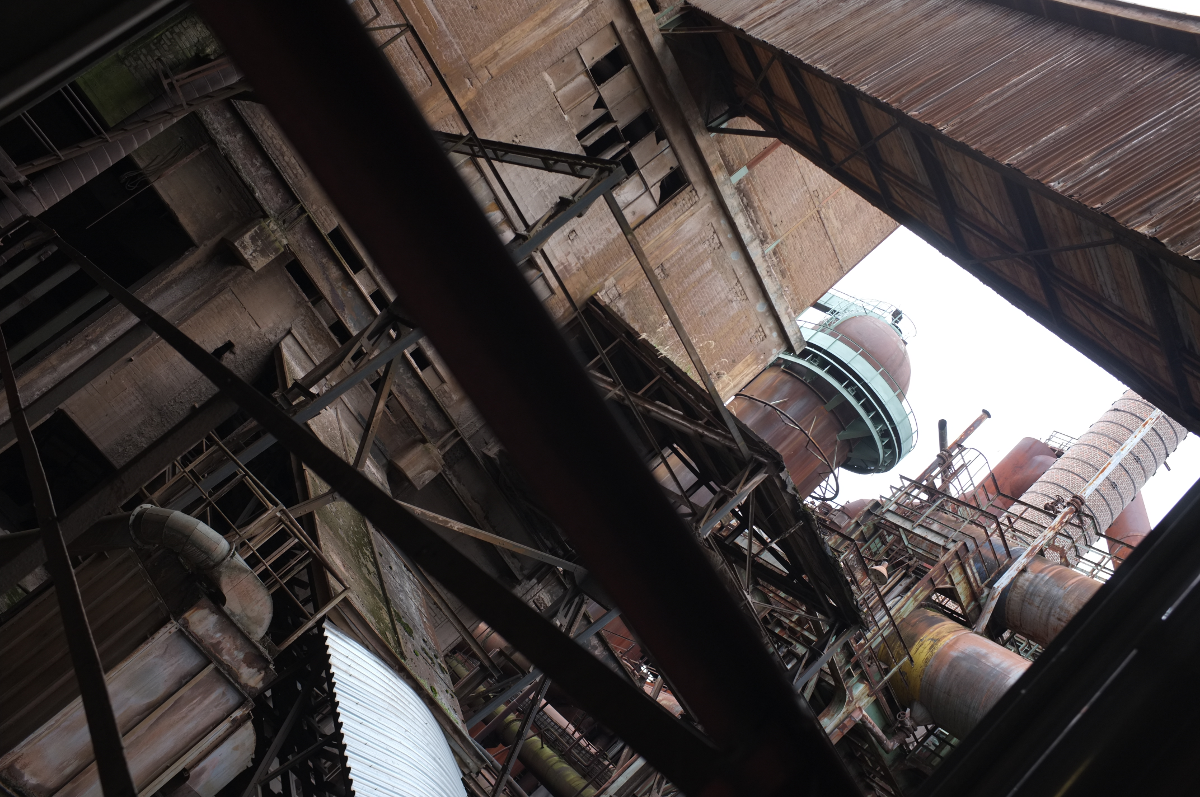
\includegraphics[width=0.7\textwidth]{Examples/example_5.png}
  \caption{Erstes Bild, Völklinger Hütte}
  \label{fig:Huette}
\end{figure}


\subsection{Wrapfigure}
Abbildung~\ref{fig:Huette} ist zwar ganz nett anzusehen, aber vielleicht sähe es eleganter aus, wenn die Abbildung 
von unserem Textabschnitt umflossen werden würde. Diese Art von Abbildungen sollte jedoch sparsam und mit großer Sorgfalt eingesetzt werden, da es zu unschönen Darstellungen kommen kann.
\blindtext
\begin{wrapfigure}{l}{0.4\textwidth}
  \centering
  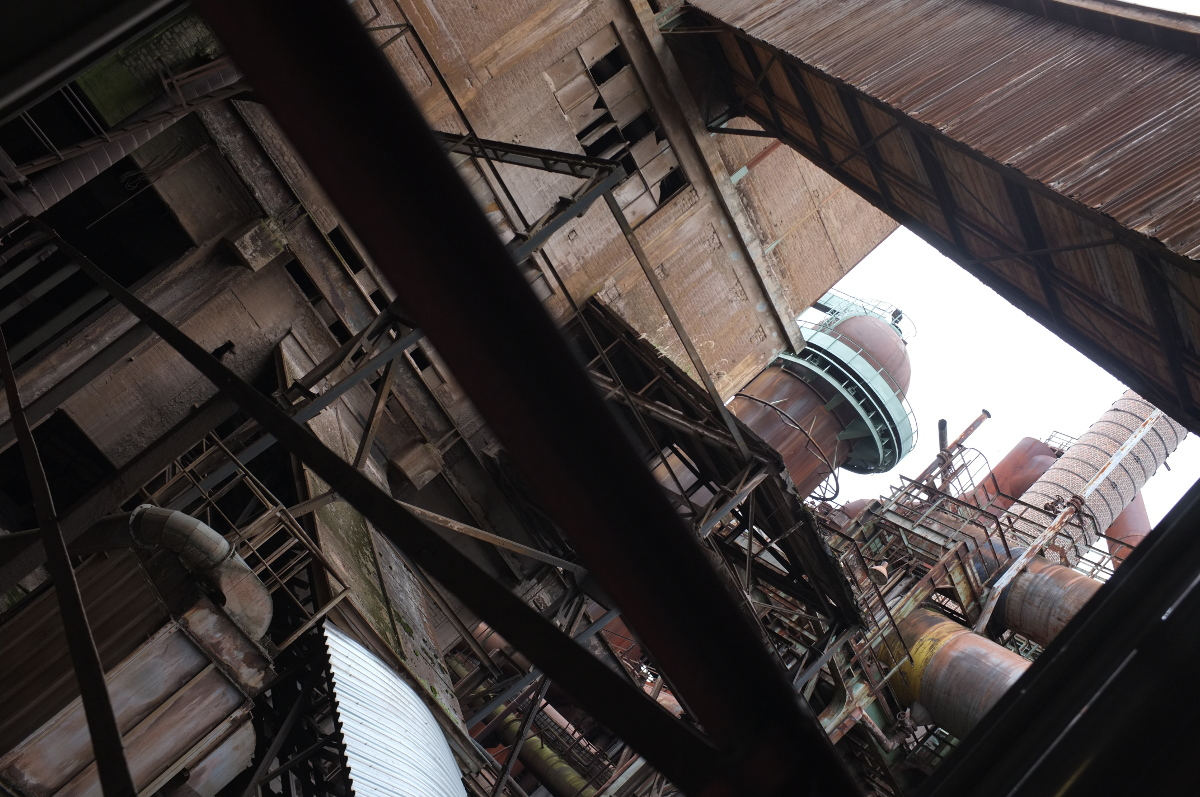
\includegraphics[width=0.4\textwidth]{Examples/example_5.jpg}
  \caption{Völklinger Hütte, *.jpg}
  \label{fig:Huette2}
\end{wrapfigure}
\blindtext


\subsection{Subfigures}
Es ist ebenso möglich, mehrere Abbildungen nebeneinander zu setzen, wie in Abbildung~\ref{fig:Beide} zu sehen ist. Eine separate Referenzierung ist auch möglich: Abbildung~\ref{subfig:abbone}.
\begin{figure}[bth]
  \subfloat[Erstes ...]{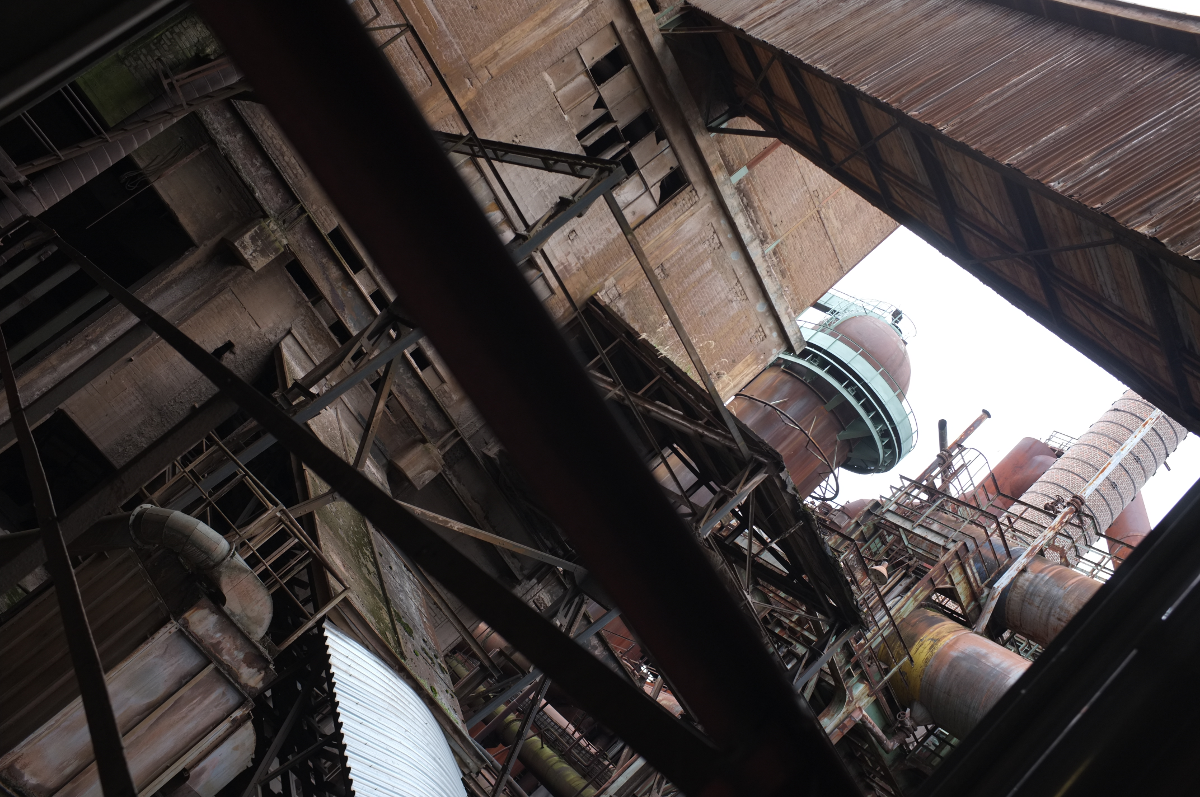
\includegraphics[width=0.49\textwidth]{Examples/example_5.png}\label{subfig:abbone}}\hfill
  \subfloat[... und zweites Bild]{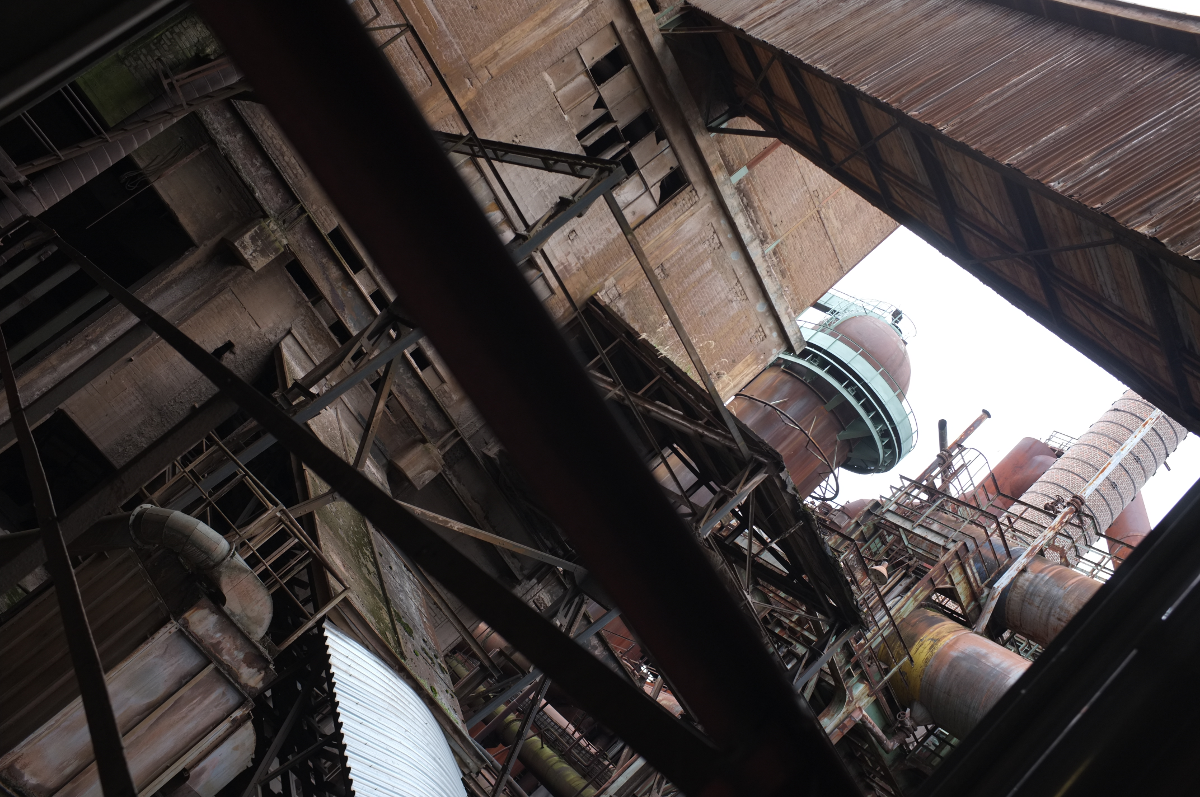
\includegraphics[width=0.49\textwidth]{Examples/example_5.png}\label{subfig:abbtwo}}
  \caption{Mehrere Abbildungen nebeneinander}
  \label{fig:Beide}
\end{figure}


\subsection{Qualitätsunterschiede}
\begin{figure}[p]
	\centering
  \subfloat[\textit{PDF}-Format]{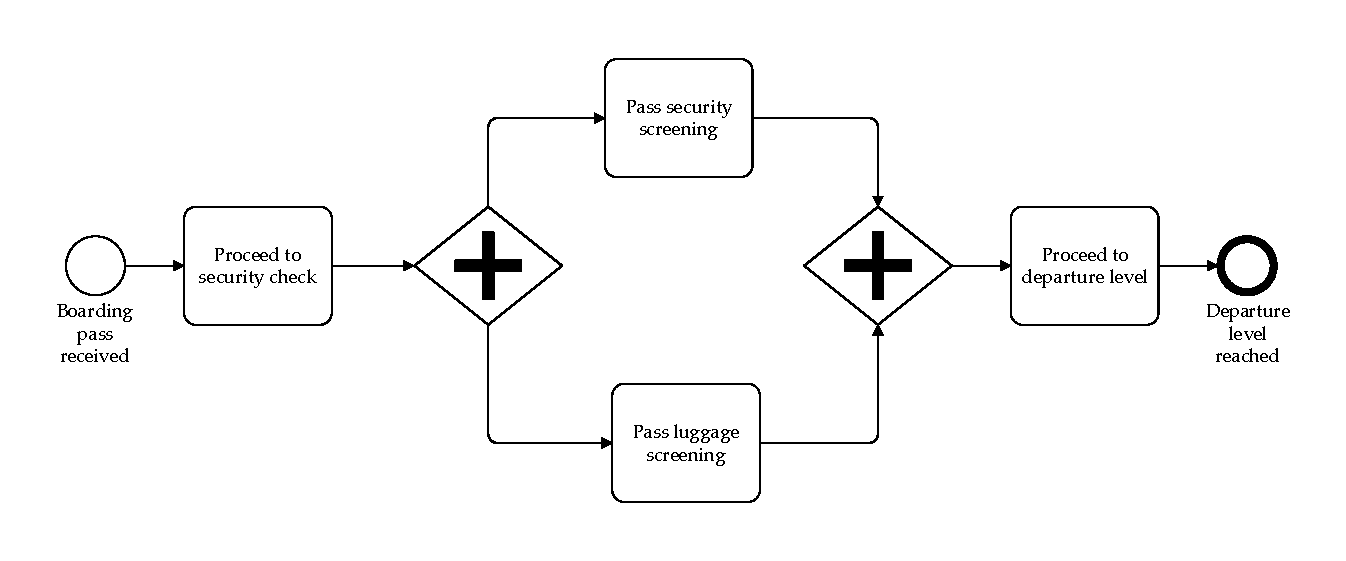
\includegraphics[width=0.65\textwidth]{Examples/bpmn.pdf}} \\
  \subfloat[\textit{JPG}-Format]{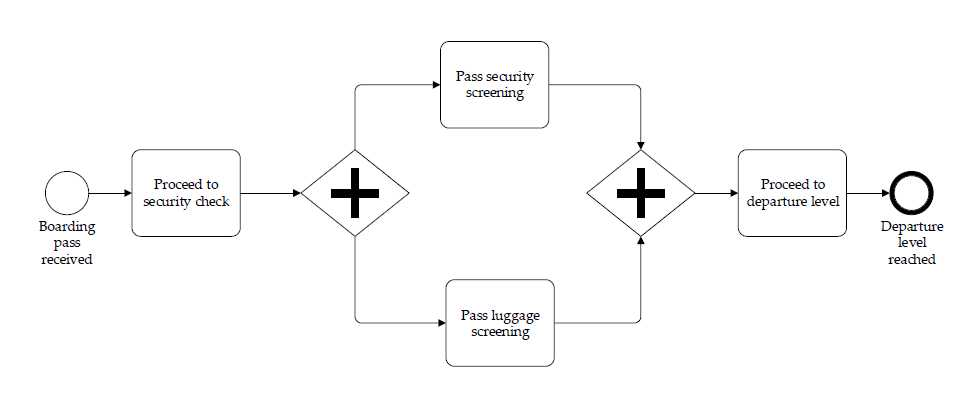
\includegraphics[width=0.65\textwidth]{Examples/bpmn.jpg}}
  \caption{Beide Formate im Vergleich}
  \label{fig:pdfvsjpg}
\end{figure}

\begin{figure}[p]
	\centering
  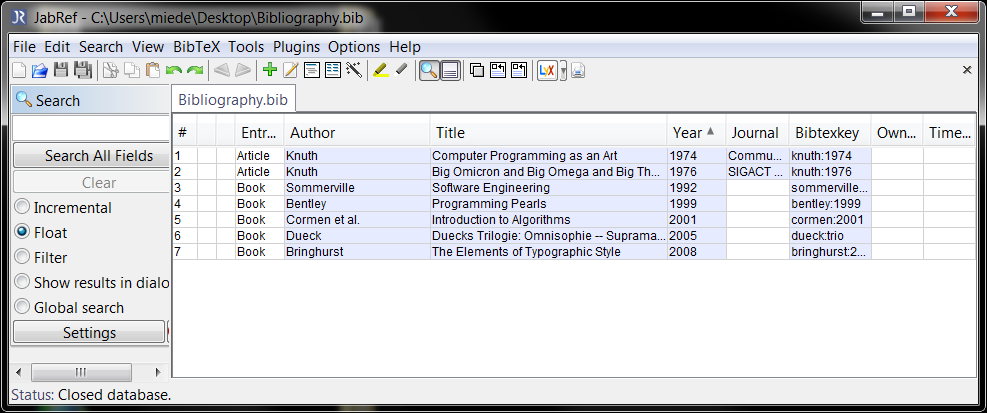
\includegraphics[width=0.65\textwidth]{Examples/jabref.png}
   \caption{\textit{PNG}-Format}
  \label{fig:pngvsjpg1}
\end{figure}

\begin{figure}[p]
	\centering
  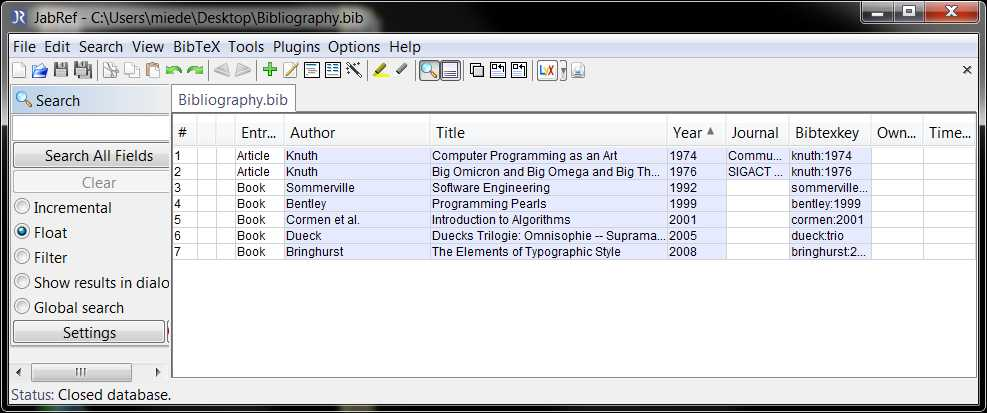
\includegraphics[width=0.65\textwidth]{Examples/jabref.jpg}
   \caption{\textit{JPG}-Format}
  \label{fig:pngvsjpg2}
\end{figure}

Leider haben die unterschiedlichen Grafikformate bedingt durch die unterschiedlichen Kompressionsverfahren einige Schwächen, insbesondere die Umwandlung in das \textit{JPG}-Format erzeugt unangenehme Artefakte im Bild. \autoref{fig:pdfvsjpg} zeigt die Unterschiede zwischen \textit{PDF-Format} und \textit{JPG-Format} im Vergleich. 

Wenn eine \textit{*.pdf}-Datei nicht infrage kommt, beispielsweise bei Screenshots, ist unbedingt das \textit{PNG-Format} vorzuziehen. 
Den Unterschied machen \autoref{fig:pngvsjpg1} und \autoref{fig:pngvsjpg2} deutlich.

\glqq Faustregeln\grqq im Umgang mit Abbildungen:
\begin{itemize}
	\item Diagramme bzw. alles, was Linien usw. enthält: \textit{PDF} (im Vektorformat).
	\item Screenshots bzw. alles, was größere gleichfarbige Flächen enthält: \textit{PNG}.
	\item Der Rest (in der Regel Fotos): \textit{JPEG}.
\end{itemize}





%*******************************
% 			Listings 		   *
%*******************************

\section{Quellcode einbinden}
Das Package \textit{lstlisting} ermöglicht es, Quellcode ansprechend in das Dokument einzubinden. Man kann Quellcode einzeilig einbinden 
mittels \lstinline{\lstinline|Quellcode|}. Dabei ist darauf zu achten, dass der Befehl einmal mit \{ \} und einmal mit | | aufgerufen werden kann, je nachdem, 
welche Zeichen im angegebenen Quelltext genutzt werden. 
Es ist auch möglich eine eigene Umgebung für Quelltext zu schaffen:

\begin{lstlisting}[caption=Erstes Listing,style=Java]
private Umgebung(int i, int k)
{
	System.out.println("Eine Funktion mit " + i + "und" + k ".");
}
\end{lstlisting}  

Wer Quelltext aus externen Dateien einbinden möchte, geht wie folgt vor:

\lstinputlisting
[caption={Externer Quellcode},style=Java]
{Examples/Code.java}

Wie genau der Quellcode formatiert und gefärbt ist, ist in \textit{htwsaar.i.mst.config.tex} hinterlegt, wobei fü verschiedene Sprachen auch eigene Styles angelegt werden
können (hier z.B. für Java).
\section{Mathematische Ausdrücke}
Mathematische Ausdrücke sind eine kleine Kunst für sich. Am allereinfachsten kann man eine Formel, wie \(a + b = c\) in den Fließtext einbinden, wobei LaTeX die Höhe der Ausdrücke der Zeile anpasst,
wie hier zu sehen \(\sum_{y=0}^{x} a\) . In einer Umgebung sieht das schon anders aus:
\begin{equation}
  \sum_{y=0}^{x} a
\end{equation}

Griechische Buchstaben:
\begin{equation}
	\alpha\beta\gamma\delta\epsilon\varepsilon\zeta\eta
	\theta\iota\kappa\lambda\mu\nu\xi\pi\varpi\rho\varrho
	\sigma\tau\upsilon\phi\varphi\chi\psi\omega
\end{equation}

Brüche:
\begin{equation}
	Ergebnis = \frac{a}{b}
\end{equation}

\begin{equation}
	\frac{\sin{\alpha}^2 + \cos{\alpha}^2}{1} = 1
\end{equation}

\begin{equation}
	\frac{-9x}{\frac{2y}{3z+2}}
\end{equation}

Text innerhalb von Formeln:
\begin{equation}
\sum_{y=1}^{n} y = \frac{n*(n+1)}{2}
\quad
\text{Gaußsche Summenformel}
\end{equation}

Hoch- bzw. Tiefstellungen:
\begin{equation}
	x_{i,j}^2
\end{equation}

\begin{equation}
	{x_{i,j}}^2
\end{equation}

\begin{equation}
	x_{n_0}
\end{equation}


Matrizen:
Matrizen werden innerhalb der mathematischen Umgebung als wiederum neue Umgebung eingebunden. Wie bei Tabellen auch werden Zeilen durch \lstinline{\\} und Spalten durch \lstinline{&} getrennt.

\begin{equation}
	\begin{pmatrix} 
		a&b\\
		c&d 
	\end{pmatrix}
\end{equation} 

\begin{equation}
	\begin{vmatrix} 
		a&b\\
		c&d 
	\end{vmatrix}
\end{equation} 

Fallunterscheidung:
\begin{equation}
	f(x) = 
	\begin{cases}
		0, &\text{falls } x < 0 \\
		1, &\text{falls } x \geq 0
	\end{cases}
\end{equation}




%############################################################
\clearpage\section{To-Do-Notes}
Um bei einer längeren Arbeit nicht den Überblick zu verlieren, an welcher Stelle es nötig ist
weiter zu arbeiten, bietet es sich an, kleine Notizen einzufügen. Das Package \textit{todonotes}
stellt eine elegante Lösung bereit, um differenziert und vielfarbig jene Abschnitte zu kennzeichnen,
die einer weiteren Bearbeitung bedürfen.

\subsection*{Beispiel für To-Do-Notes}
Dies hier ist ein Blindtext zum Testen von Textausgaben. Wer diesen Text liest, ist selbst
\todo{Plain todonotes.} schuld. Der Text gibt lediglich den Grauwert der Schrift an. Ist das wirklich so? Ist es
gleichgültig, ob ich schreibe: Dies ist ein Blindtext? oder Huardest gefburn? Kjift?
mitnichten! Ein Blindtext bietet mir wichtige Informationen. An ihm messe ich die Les-
barkeit einer Schrift, ihre Anmutung, \todo{Plain todonotes.}wie harmonisch die Figuren zueinander stehen
und prüfe, wie breit oder schmal sie läuft. Ein Blindtext sollte möglichst viele verschie-
dene Buchstaben enthalten und in der Originalsprache gesetzt sein. Er muss keinen
Sinn ergeben, sollte aber lesbar sein.\todo[nolist]{Todonote that is only shown in the margin and not in
the list of todos.}%
Fremdsprachige Texte wie Lorem ipsum dienen
nicht dem eigentlichen Zweck, da sie eine falsche Anmutung vermitteln. Dies hier ist
ein Blindtext zum Testen von Textausgaben. Wer diesen Text liest, ist selbst schuld. 

\todo[inline]{A very long todonote that certainly will fill more
than a single line in the list of todos. Just to make sure let's add
some more text \ldots}

Der Text gibt lediglich den Grauwert der Schrift an. Ist das wirklich so? Ist es gleichgültig,
ob ich schreibe: Dies ist ein Blindtext? oder Huardest gefburn? Kjift? mitnichten!
\todo[noline]{A note with no line back to the text.}
Ein Blindtext bietet mir wichtige Informationen. An ihm messe ich die Lesbarkeit einer
Schrift, ihre Anmutung, wie harmonisch die Figuren zueinander stehen und prüfe, wie
\todo[caption={A short entry in the list of todos}]{A very long
todonote that certainly will fill more than a single line in the
list of todos \ldots}
breit oder schmal sie läuft. Ein Blindtext sollte möglichst viele verschiedene Buchstaben
enthalten und in der Originalsprache gesetzt sein. Er muss keinen Sinn ergeben, sollte
aber lesbar sein. Fremdsprachige Texte wie Lorem ipsum dienen nicht dem eigentlichen Zweck, 
da sie eine falsche Anmutung vermitteln.
\missingfigure{A figure I have to make \ldots}

%Nummerierte ToDo-Notes
\todox{Erste Nummer...}
\todox{Zweite Nummer...}

%Alles To-Dos als Liste ausgegeben
Nachfolgend wird noch eine Liste aller To-Dos auf einer separaten 
Seite ausgegeben.
%\begingroup
	%\let\clearpage\relax
	%\let\cleardoublepage\relax
	\listoftodos
%\endgroup 


 		% Abschlussarbeit geht!
\cleardoublepage\chapter{Einleitung}
\label{ch:Einleitung}


\section{Problemstellung}
Die Firma HYDAC Systems und Services GmbH entwickelt derzeit ein System zum erfassen, verarbeiten und auswerten von Messwerten und Prozessdaten in Echtzeit. Allgemein ist solch ein System auch unter dem Begriff Condition Monitoring bekannt und ermöglicht es Prozesse zu überwachen, zu planen und gegebenenfalls zu optimieren. Es wird demnach zur Prozessoptimierung verwendet und erhöht die Verfügbarkeit von Anlagen. Im Rahmen der Machbarkeit und Untersuchung unterschiedlicher Herangehensweisen, ist es für die Firma interessant wie Studenten der Hochschule htwsaar ein Condition Monitoring System anhand gegebener Anforderungen konzipieren würden.

\section{Zielsetzung}
Das Ziel dieser Arbeit soll es sein, einen Architekturentwurf für ein Condtion Monitoring auszuarbeiten, welcher unter Anwendung moderner Architekturansätze zu gestalten ist. Wichtig ist es auch, das die Vorgaben der Firma mit in das Konzept fließen.

\section{Stakeholder}

\section{Gliederung}
Das erste Kapitel gibt einen Überblick über die Themen, welche folgend in der Dokumentation ausformuliert sind. Im Kapitel \ref{ch:Anforderungsanalyse}, werden sowohl die funktionalen, als auch die nicht-funktionalen definiert und erörtert. Es schafft Klarheit darüber wer, warum und wozu solch ein System benötigt wird und definiert die zentralen Merkmale. Das \ref{ch:Konzept} befasst sich danach mit den aus Kapitel \ref{ch:Anforderungsanalyse} gestellten Anforderungen und beschreibt ein mögliches Konzept nach Kriterien. Kapitel Im letzten Kapitel \ref{ch:Fazit} werden wir das Vorgehen abschließend beurteilen und einen Ausblick wagen. 
\cleardoublepage\chapter{Einflussfaktoren}
\label{ch:Einflussfaktoren}
\section{Organisatorische Einflussfaktoren}
\section{Technische Einflussfaktoren} 
\cleardoublepage\chapter{Kontextabgrenzung}
\label{ch:Kontextabgrenzung}
%siehe vorlesunng 
\cleardoublepage\chapter{Lösungsstrategie}
\label{ch:Lösungsstrategie}
In diesem Kapitel werden nun die grundlegenden Entscheidungen und Lösungsansätze unseres Entwurfs vorgestellt. In den folgenden Technologieentscheidungen werden die Entscheidungen der Architektur festgelegt.  
\begin{itemize}
	\item Entkopplung der Datenbanken zur Fachdomäne mittels Schnittstellenklassen und der Nutzung von 2 separaten Datenbanken(Qualitätsziel: Performance)
	\item Verringerung der Flexibilität, durch Verzicht auf Abstraktionsschichten(Qualitätsziel: Performance)
	\item Zyklische redundante Speicherung ausgewählter Daten und bereitstellen von Hardware-Backupsystemen (Qualitätsziel: Verfügbarkeit)
	\item Einsatz naher Programmiersprachen C und C++ (Qualitätsziel: Performance)
	\item Keine Verteilung des Systems(Qualitätsziel: Performance)
	\item Fehlererkennung durch kontinuierliches Versenden von Heartbeat(Qualitätsziel: Verfügbarkeit)
	\item Systemzustand wird periodisch gespeichert um im Fehlerfall zurücksetzen zu können(Qualitätsziel: Verfügbarkeit) 
	\item Benutzerschnittstelle soll Datenobjekte durch Masken erzeugen und manipulieren können. (Qualitätsziel: Nutzbarkeit) 
	\item Die Benutzerschnittstelle läuft auf der Zielplattform in einem Web-Client und wird über den nginx-Webserver verwaltet (Qualitätsziel: Nutzbarkeit)
	\item Nutzung von Capt'n Proto beim Serialisieren und Deserialisieren von Daten (Qualitätsziel: Performance)
\end{itemize}  
\cleardoublepage\chapter{Bausteinsicht}
In diesem Kapitel zeigen wir den Aufbau des Condition Monitoring Systems. Es werden dabei die grundlegenden Pakete, Programmstrukturen und Komponenten beschrieben.
\section{Ebene 1}
Die Bausteine der ersten Ebene sind zu implementierende Einheiten. Dazu gehören die Daten IO-Module, die Controller-Module und das Applikation-Presenter-Modul. 
Die verschiedenen Module enthalten unterschiedliche Architekturstile, wodurch unser Gesamtsystem eine heterogene Softwarearchitektur aufweist. Jedes Modul verantwortet einen Teil der Gesamtfunktionalität. Anhand dieser werden die folgenden Ebenen um weitere Einheiten erweitert. Die folgende Grafik gibt einen ersten Überblick über das System.
\begin{figure}[h]
	\centering
	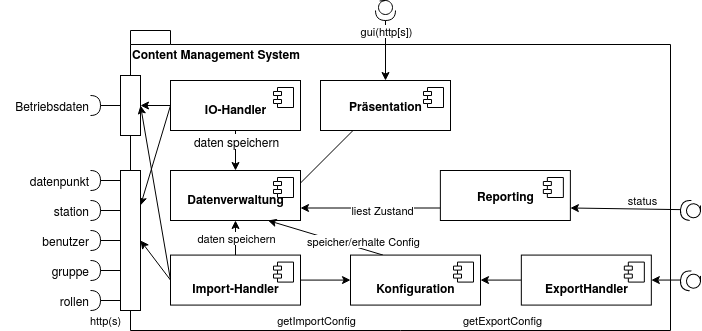
\includegraphics[width=1.0\textwidth]{Graphics/bausteinansicht_ebene_1.png}
	\caption{Bausteinsicht Level 1}
	\label{fig:bausteinsichtlvl1}
\end{figure}

Das Architekturziel hohe Performance zu gewährleisten, wird von der Komponente IO-Modul verantwortet.
Das Controller-Modul, stellt sicher, dass das Architekturziel der Verfügbarkeit eingehalten wird. 
Das Applikation-Präsenter-Modul verantwortet, dass das Architekturziel der Benutzerfreundlichkeit eingehalten wird.
Die folgenden Abschnitte beschreiben die in der Abbildung dargestellten Einheiten von links nach rechts.  
\subsection{IO-Module}
\begin{table}
	\begin{tabularx}{\textwidth}{X X}
		\hline
		 Zweck/Verantwortlichkeit & Das Modul nimmt über Außenschnittstellen Daten von Fremdsystemen entgegen und ist für deren korrekte persistente Speicherung verantwortlich  \\
		 \hline
		 Schnittstellen intern & Speichert Konfigurationsdaten und Rohdaten in Datenbank \\
		 \hline
		 Schnittstellen extern & Eingang von Rohdaten(csv, json, binär) und Konfigurationsdaten (Datenpunkt, Station, Benutzer, Gruppe, Rollen, Regeln) \\
		 \hline
	\end{tabularx} 
	\caption{Fachliche Kontextabgrenzung der Kommunikationspartner}
	\label{tab:FachlicheKontextabgrenzungDerKommunikationspartner}
\end{table}

\subsection{Controller-Module}
\begin{table}[th]
	\begin{tabularx}{\textwidth}{X X}
		\hline
		Zweck/Verantwortlichkeit & Verwaltet sämtliche Daten und beinhaltet Funktionsblöcke die Verwaltungsoperationen Lesen, Schreiben und Löschen bereitstellen. \\
		\hline
		Schnittstellen intern & Liefert \\
		\hline
	\end{tabularx} 
	\caption{Fachliche Kontextabgrenzung der Kommunikationspartner}
	\label{tab:FachlicheKontextabgrenzungDerKommunikationspartner}
\end{table}

\subsection{Applikation-Präsenter-Modul}
\begin{table}[th]
	\begin{tabularx}{\textwidth}{X X}
		\hline
		Zweck/Verantwortlichkeit & Anzeigeoberfläche für Benutzer \\
		\hline
		Schnittstellen intern & Nutzt den Webserver des Controller-Moduls\\
		\hline
	\end{tabularx} 
	\caption{Fachliche Kontextabgrenzung der Kommunikationspartner}
	\label{tab:FachlicheKontextabgrenzungDerKommunikationspartner}
\end{table}
%Damit die die vielen Fremdsysteme und Maschinen mit unserer Software kommunizieren können, benötigen wir Implementierungen aller Protokolle in C++. Für CAN bzw. CANopen hat Alex eine Bibliothek in seiner Bachelorarbeit geschrieben. Für TCP/RTU nutzen wir Qt, für S7 gibt es Snap7. Die Hydac hat ihre eigene API und Bibliothek für die eigenen HFI-MM und HFI-CM Protokolle. Zu guter Letzt serialisieren wir WebSocket und HTTP mit Capn Proto. Alle Bibliotheken ermöglichen das einfache Abspeichern in den Wide-Column-Store oder bereiten es zumindest vor. Dafür werden eine DatenpunktID und StationsID der Maschine mit dem Wert und dem Zeitstempel gespeichert. Da diese Daten komplett ungeprüft in die Datenbank einfließen, muss ein weiterer Baustein alle Einträge überprüfen und Messfehler oder kritische Werte direkt in der Weboberfläche anzeigen. Dass die Überprüfung eventuell etwas langsamer als der Datenstrom in die Datenbank sein kann, ist an sich nicht schlimm, da die Anwendung in Produktionspausen aufholen und die noch ungeprüften Daten währenddessen verarbeitet.In der relationalen Datenbank befinden sich dann die DatenpunktIDs mit ihren Typen und Formaten, damit man ein Schema zur Darstellung im Interface hat. zusätzlich zu den Nutzer- und Rechtedaten gibt es auch noch eine Tabelle, die Regeln für die Datenpunkte abbildet.\\
\clearpage
\section{Ebene 2}
\begin{figure}[h]
	\centering
	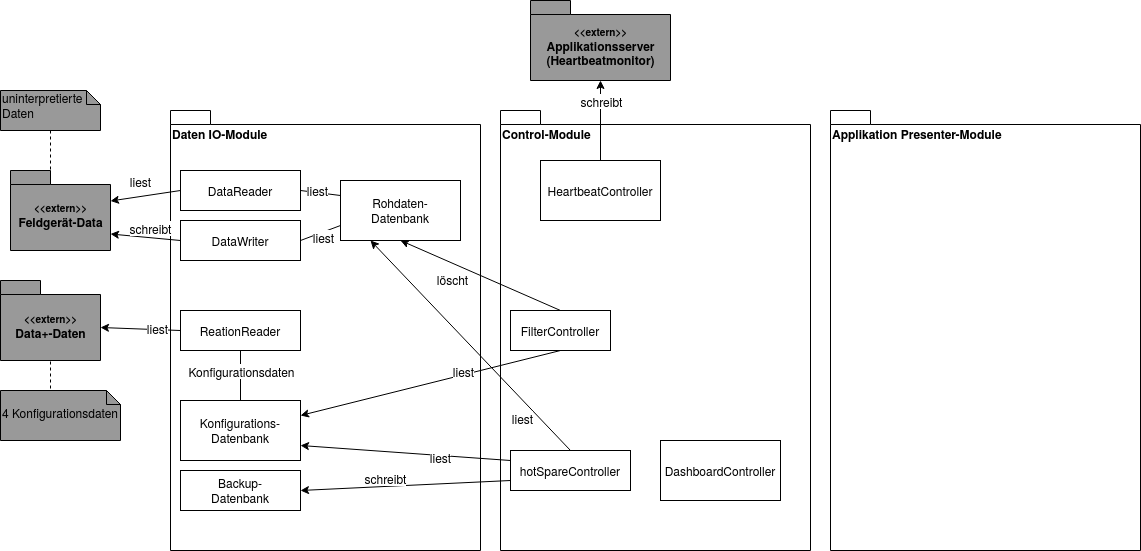
\includegraphics[width=1\textwidth]{Graphics/bausteinansicht_ebene_2.png}
	\caption{Bausteinsicht Level 2}
	\label{fig:bausteinsichtlvl2}
\end{figure}
Das Webinterface hat zu beiden Datenbanken eine Verbindung und kann auch die API des Filtermoduls mitbenutzen. In der Nutzeroberfläche wird zwischen einem administrativem und einem anwendungsspezifischen Teil unterschieden. In letzterem werden nur Daten und Statistiken aufbereitet angezeigt, während die Rechtevergabe und Feineinstellung in der Administratoroberfläche stattfindet.  
\cleardoublepage\chapter{Laufzeitsicht}
\label{ch:Laufzeitsicht}

Szenario: Daten Werden übergeben und dann simuliert
\begin{figure}[tbh]
    \centering
    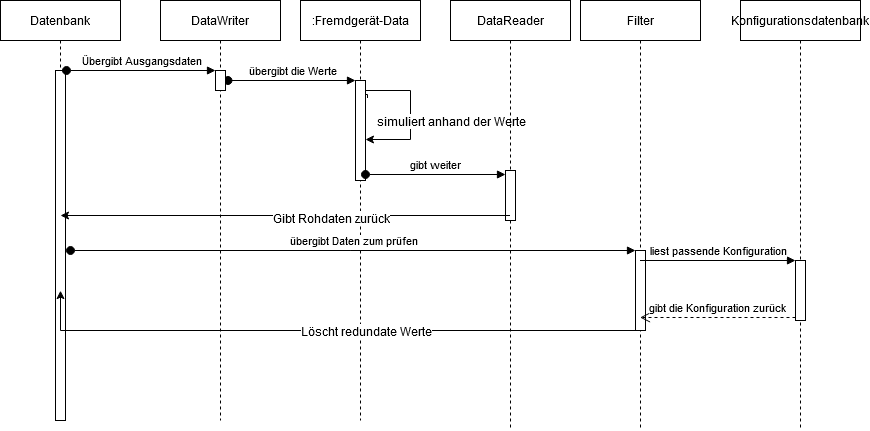
\includegraphics[width=0.7\textwidth]{Graphics/Laufzeit_Rohdaten.png}
    \caption{Laufzeitsicht für Rohdaten}
    \label{fig:Laufzeit}
  \end{figure} 
\cleardoublepage\chapter{Verteilungssicht}
\label{ch:Verteilungssicht}
In der Verteilungssicht werden wir uns nun mit der Infrastruktur unserer Architektur befassen. Sie veranschaulicht den technischen Ablauf in unserem System und spiegelt dies in Form der gewählten Hardwarekomponenten sowie des in Abbildung \ref{fig:verteilung} veranschaulichten UML-Deployment Diagram wieder.

\begin{figure}[h]
	\centering
	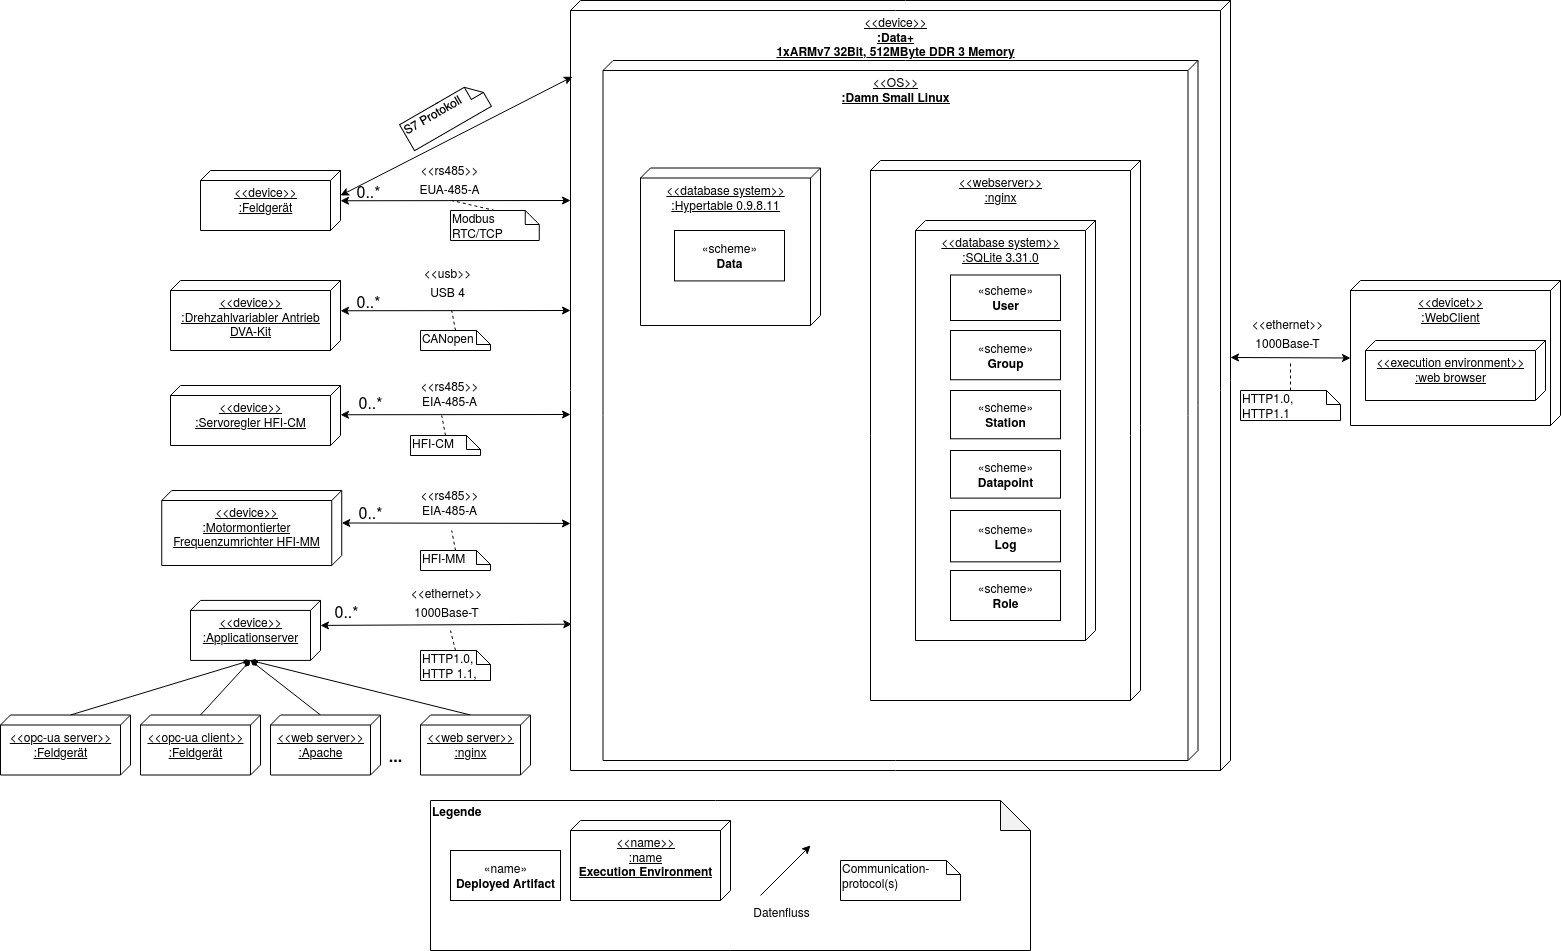
\includegraphics[width=1.1\textwidth]{Graphics/verteiler.png}
	\caption{Verteilungssicht der Anwendung}
	\label{fig:verteilung}
\end{figure}

Wie in der Abbildung zu sehen ist, besitzt das Device zwei Datenbanksysteme unterschiedlichen Typs. Zum einen eine relationale SQLite-Datenbank zum erfassen und verwalten von Konfigurationen, Systemzustand und Benutzerverwaltung, als auch eine Wide-Column-Store Hypertable-Datenbank zum speichern von eingehenden Betriebsdaten.
Die Funktionalität einer Weboberfläche wird mittels ngnix-Webserver, der auf die Daten der relationalen Datenbank zugreift bereitgestellt. Jedes der externen Geräte wird an einen der möglichen physikalischen Ports angebunden. Da hier unter anderem Bussysteme verwendet werden, muss davon ausgegangen werden, das mehrere Geräte auf einem Physikalischen Port angeschlossen sein können. Dabei veranschaulicht die Abbildung \ref{fig:verteilung} nicht die physikalisch möglichen Anschlüsse, sondern die logischen. An das System können verschiedene Bussysteme und Netze gleichzeitig angeschlossen werden. Die Anzahl der mit dem Device verbundenen Geräte wird dabei lediglich durch die Bus-/Netzwerkspezifische Maximalgröße und die Anzahl physikalischer Ports beschränkt. Allgemein unterstützt das System die Kommunikation mit den Bussystemen Modbus RTC/TCP, CAN/CANopen, HFI-CM, HFI-MM und Protokollen S7, HTTP1.0 und HTTP1.1.    
\cleardoublepage\chapter{Entwurfsentscheidungen}
\section{Persistenz}
Die Art und Weise, wie Daten beständig und dauerhaft in dem System gespeichert werden können ist mit das Herzstück eines Condition Monitoring Systems. Das Hauptaugenmerk dabei ist es diese Daten in einer besonders hohen Geschwindigkeit zu speichern, da ein besonders hohes Datenvolumen möglich und vom Anwender gewünscht ist. Speichermodelle mit langen Speicherzeiten sind den Anforderungen demnach ungenügend und eignen sich nicht für die Speicherung von Daten. Wide-Column-Store Datenbanken würden sich als mögliches Speichermodell anbieten. Sie sind eine Erweiterung von Key-Value-Store Datenbanken und speichern ihre Daten in einer Struktur, ähnlich dem Schema einer Tabelle ab. Der Schlüssel ist ein Bytearray und der Wert besteht aus Paaren von Spaltenname und -werten. Im Gegensatz zum relationalen Modell gibt es kein fixes Schema. Ein solches System ist zum Beispiel Hypertable, das mit einem geringen Speicherplatzbedarf sich optimal eignet. Nach eigenen Angaben soll das System sich sogar um die Konsistenz der Daten kümmern, während sich viele NoSQL-Datenbanken mit einer vermeintlichen Konsistenz der Daten begnügen.
\subsection{NoSQL-Datenbanksystem}
Im Vergleich standen drei Datenbanksysteme desselben Typs als Vergleich gegenüber. Das Datenbanksystem von Orcale Berkeley DB gibt es schon seit 1994 und wurde je nach Edition in C, C++ oder Java implementiert. Es handelt sich dabei um einen Key-Value Speicher, der XML-Unterstützung bietet, SQL und sekundäre Indexierung kann. Die Datenbank wird nach dem ACID-Prinzip gefüllt und ist trotzdem noch sehr schnell bzw. und mit der richtigen Konfiguration auch komplett parallel nutzbar.
Das Redis ist eine beliebte Datenbanksoftware, die seit 2009 auf dem Markt ist. Sie ist ein in C geschriebener Key-Value-Speicher, der eine große, aber keine vollständige Konsistenz der Daten verspricht. Dafür ist der Zugriff komplett parallel und kann durch einige Einstellungen auch stark konsistent werden. Allerdings ist Konsistenz eine starke Anforderung und verpflichtend für die Datenbank. Das wie eben schon erwähnte Projekt Hypertable wurde im März 2016 eingestellt und basiert auf BigTable und sowie Daten. Es wurde in C++ geschrieben und ist ein schemafreies System. Die Vorteile liegen in der sofortigen Konsistenz der Daten und der Möglichkeit gleichzeitig lesen und schreiben zu können. Der große Nachteil ist, dass es keine Updates mehr gibt, da das Projekt nicht fortgesetzt wird. Trotzdem ist diese Software in den Schreibvorgängen am schnellsten, wie folgendes Benchmark zeigt \url{https://wiki.volution.ro/Dehems/Benchmarks/Results}.
\subsection{SQL-Datenbanksystem}
Für die anderen Datensätze wie Benutzer-, Rechte- und Komponentenverwaltung haben wir uns für SQLite entschieden. Die Datenbank benötigt für den Betrieb äußerst wenig Ressourcen und Leistung und benötigt so beispielsweise gerade mal ca. 350 kByte an Speicher. Hinzu kommt, das durch die einfache Integration und Verwaltung das System schnell integriert und verteilt werden kann. Für ein Benchmark ist folgendes Seminar in Datenbanksysteme der FHO HSR herangezogen worden \cite{MorierWeber2011}.
\subsection{Serialisierung Capn Proto}
Da wir mit einem System arbeiten, das eingehende wie ausgehende Daten, in dem System fachterminologisch als Datenpunkt bezeichnet, verarbeitet und mit programminternen sowie /-externen Einheiten kommuniziert, muss bekanntlich auch eine Serialisierung dieser Daten erfolgen.  Bei einer Reihe zur Verfügung stehender Serialisierungstechnologien ist es für das Produkt nötig die Vor- und Nachteile der jeweils einzelnen abzuwägen. Da es für das System von großer Wichtigkeit ist mit einem möglichst großen Datendurchsatz performant umgehen zu können, können textbasierte Serialisierungstechniken wie JSON, XML, YAML usw. kategorisch abgelehnt werden. Der Grund dafür ist, dass im Allgemeinen ein zu großer Speicherbedarf benötigt wird, was zur Folge hat, dass die Serialisierungszeit und damit auch die Laufzeit stark ansteigt.\\ 
Eine Möglichkeit die Laufzeit zu verringern wäre eine adhoc single String Technik zu verwenden. Diese muss jedoch redundant für jede Sprache geschrieben werden, was uns in der Portierbarkeit einschränken würde.\\
Die nach unserer Meinung nach beste Lösung für dieses Problem wäre es demzufolge eine schemagesteuerte binäre Serialisierungstechnik zu verwenden. Zum Einsatz soll Capn Proto verwendet werden. Durch dessen flexible Schemadefinition lässt sich im Vergleich zu den anderen Portierbarkeit erhöhen, da dieses Framework den Serialisierungscode anhand der Schemadefinition selbst erzeugt. Die binäre Darstellung der Daten erlaubt zudem eine deutlich effizientere Übertragung der Daten. Capn Proto ist im Vergleich zu Protobuf fast doppelt so schnell, siehe \url{https://github.com/ChrisMacNaughton/proto_benchmarks/}. Die Bibliotheken sind einfach zu nutzen und in C++ geschrieben.
\subsection{Parallelisierung}
Damit alle Systeme und Komponenten zeitgleich ihre Aufgaben erfüllen können, wird die Software in Micro Services aufgebaut, die unabhängig voneinander parallel arbeiten können.\\
Weitere Vorteile liegen in der unabhängigen Entwicklung, Implementierung und Wartung der einzelnen Bausteine. Allerdings wird dadurch auch ein Load Balancer nötig, der die Ressourcen der Hardware nach den Anfragen auf die einzelnen Prozesse verteilt. 
\subsection{Fehlererkennung}
Pings oder ICMP Request/Replies werden zwar oft genutzt um zu sehen, ob ein Server noch online ist, aber da ICMP betriebssystemspezifisch implementiert ist und in manchen Sicherheitsrichtlinien deaktiviert sein muss, kann man das hier nicht für eine dauerhafte Taktik verwenden. Außerdem erhält man keine Einsicht darüber, ob ein Programm auf der Maschine ausgeführt ist, was in unserem Fall aber wichtig wäre. 
\\
Mit Hilfe von Monitoring kann man die Antwortzeiten und die Uptimes von allen Anwendungen eines Servers abfragen und darstellen. Diese Methode ist zielführender, braucht allerdings eine zusätzliche Schnittstelle, die nicht immer bereitgestellt werden kann. Auch verbraucht sie einige Ressourcen und die Abfrage kann bzw. sollte nicht in zu kurzen Zeitintervallen stattfinden. 
\\
Heartbeat ist eine periodischer Nachrichtenaustausch zwischen einem Prozess und einem Kontrollsystem. Da unsere Anwendung in Echtzeit große Datenmengen bewältigen muss, ist es wichtig, dass der Heartbeat schnell und einfach gesendet und empfangen wird um keine anderen Daten/Datenverarbeitungen zu behindern. 
Mit Hilfe von Condition Monitoring kann man zum Beispiel bei einer Maschine aus Sensordaten Schwingungen und Temperaturen erfassen, die evtl. für Ausfälle sorgen. Um das bei unserem Server anzuwenden, muss man die CPU-Temperatur überwachen und ggf. den Serverschrank weiter runterkühlen um Ausfälle zu vermeiden. 
Voting ist nicht nur prozessorlastig, sondern wird am besten auch auf mehreren Geräten gleichzeitig ausgeführt was langsam und kostenintensiv ist, daher verwerfen wir diese Möglichkeit.
\\
Zeitstempel kann man einfach in die Datenbank einpflegen um evtl. fehlerlastige Zeiten herauszufinden und zu löschen oder zu korrigieren. Eine größere Validierung wird wieder zu CPU-lastig und kann daher nicht direkt beim Speichern der Daten durchgeführt werden.\\
Aus Kostengründen müssen wir auch alle Wiederherstellungsmaßnahmen, die Redundanz beinhalten leider ausschließen, da das Budget zu klein gesetzt wurde. Daraus folgt, treten Softwarefehler ein, muss man mit Hilfe von Hotfixes und bei Hardwarefehlern mit einem Austauschgerät arbeiten. Außerdem kann man bei Exceptions, die zur Laufzeit auftreten den jeweiligen Stacktrace mit der dazugehörigen Eingabe an eine Kontrollstelle abspeichern. Sobald eine kritische Anzahl an Exceptions pro Minute/Stunde auftritt muss der Fehler in der Software gepatcht werden. Im Softwaredesignprozess muss dabei darauf geachtet werden, dass Exceptions immer gehandelt werden und das auch in sehr ungewöhnlichen oder gar unmöglichen Fällen um in jedem Szenario handlungsfähig zu bleiben.
\\
Abschließend haben wir uns für eine Kombination aus Condition Monitoring, Exception Handling und Zeitstempel entschieden, weil diese kaum Leistung benötigen und Kosten verursachen. Hotfixes für Ausfälle sind gerade im Pilotbetrieb erstmal günstiger als redundante Hardware und komplexe Monitoringtools. Diese können bei Bedarf in einer späteren Variante auf besserer Hardware eingebaut werden.
  
\cleardoublepage\chapter{Qualitätsszenarien}
\label{ch:Qualitaetsszenarien}


\begin{figure}[tbh]
  \centering
  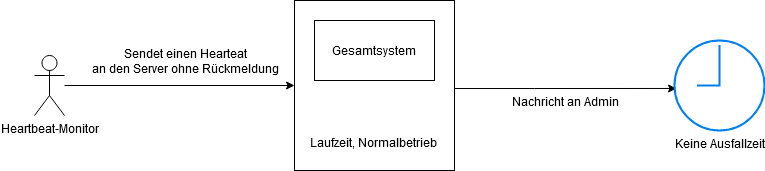
\includegraphics[width=0.7\textwidth]{Graphics/Verfuegbarkeit.png}
  \caption{Verfuegbarkeits-Szenario}
  \label{fig:Qualitaet1}
\end{figure}

Verfuegbarkeits-Szenario\\
Source of Stimulus: Heartbeat Monitor\\
Stimulus: Sendet einen Heartbeat an den Server ohne Rückmeldung\\
Environment: Laufzeit, Normalbetrieb\\
Component: Gesamtsystem\\
Response: Nachricht an Admin\\
Response Measure: Keine Ausfallzeit\\

Heartbeat an eine Serverkomponente geschickt.  Dadurch haben wir ein Verteiltes System



\begin{figure}[tbh]
  \centering
  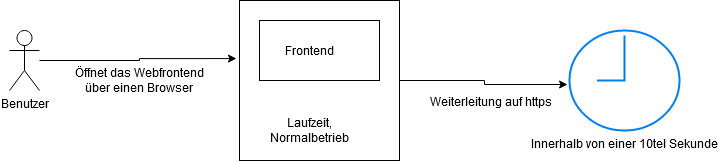
\includegraphics[width=0.7\textwidth]{Graphics/Sicherheit.png}
  \caption{Sicherheit-Szenario}
  \label{fig:Qualitaet2}
\end{figure}


Sicherheits-Szenario\\
Source of Stimulus: Benutzer\\
Stimulus: Öffnet das Webfrontend über einen Browser über http\\
Environment: Laufzeit, Normalbetrieb\\
Component: Frontend\\
Response: Weiterleitung auf https\\
Response Measure: Daten sind verschlüsselt\\




\begin{figure}[tbh]
  \centering
  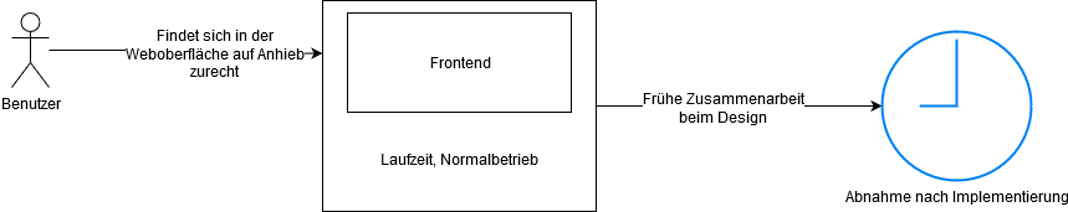
\includegraphics[width=0.7\textwidth]{Graphics/Nutzbarkeit.png}
  \caption{Nutzbarkeit-Szenario}
  \label{fig:Qualitaet3}
\end{figure}



Nutzbarkeits-Szenario
Source of Stimulus: Benutzer\\
Stimulus: Öffnet das Webfrontend\\
Environment: Laufzeit, Normalbetrieb\\
Component: Frontend\\
Response: Öffnet das Tutorial / Hilfe-Meldung\\
Response Measure: Neue Nutzer haben einen guten Einstieg in der Software\\





\begin{figure}[tbh]
  \centering
  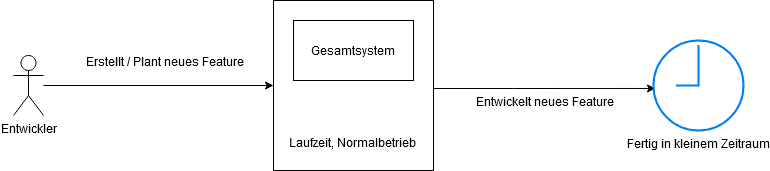
\includegraphics[width=0.7\textwidth]{Graphics/Erweiterbarkeit.png}
  \caption{Erweiterbarkeits-Szenario}
  \label{fig:Qualitaet3}
\end{figure}


Erweiterbarkeits-Szenario\\
Source of Stimulus: Entwickler\\
Stimulus: Erstellt / Plant neues Feature\\
Environment: Laufzeit, Normalbetrieb\\
Component: Gesamtsystem\\
Response: Implementierung ohne negativen Sideeffects\\
Response Measure: Implementierung innerhalb einer Woche \\



\begin{figure}[tbh]
  \centering
  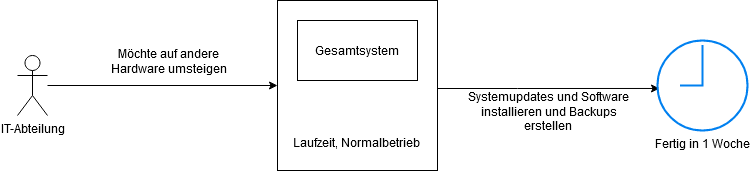
\includegraphics[width=0.7\textwidth]{Graphics/Portierbarkeit.png}
  \caption{Portierbarkeit-Szenario}
  \label{fig:Qualitaet4}
\end{figure}



Portierbarkeits-Szenario\\
Source of Stimulus: IT-Abteilung\\
Stimulus: Möchte auf andere Hardware umsteigen\\
Environment: Laufzeit, Normalbetrieb\\
Component: Gesamtsystem\\
Response: Systemupdates und Software installieren und Backups erstellen \\
Response Measure: Fertig in 1 Woche\\




\begin{figure}[tbh]
  \centering
  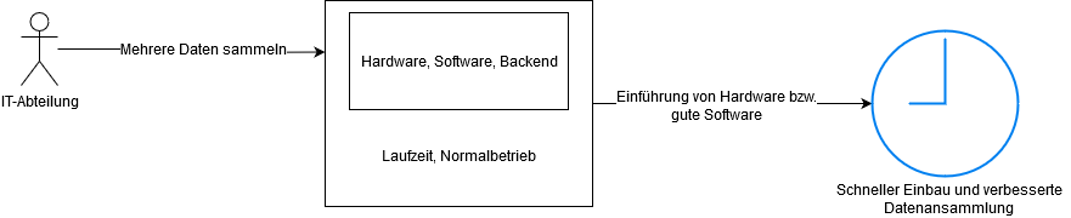
\includegraphics[width=0.7\textwidth]{Graphics/Effizienz.png}
  \caption{Effizienz-Szenario}
  \label{fig:Qualitaet5}
\end{figure}



Effizienz-Szenario\\
Source of Stimulus: Entwickler\\
Stimulus: Mehrere Daten sammeln\\
Environment:Laufzeit, Normalbetrieb\\
Component: Hardware, Software, Backend\\
Response: Einführung von Hardware, bzw. gute Software um Datenpunkte zu sammeln\\
Response Measure: Schneller Einbau und verbesserte Datensammlung\\




\begin{figure}[tbh]
  \centering
  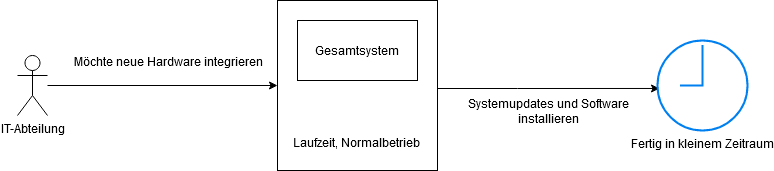
\includegraphics[width=0.7\textwidth]{Graphics/Hardware.png}
  \caption{Hardware-Szenario}
  \label{fig:Qualitaet6}
\end{figure}


Hardware-Szenario\\
Source of Stimulus: IT-Abteilung\\
Stimulus: Möchte neue Hardware integrieren\\
Environment:Lautzeit, Normalbetrieb\\
Component: Gesamtsystem\\
Response: Systemupdates und Software installieren\\
Response Measure: Fertig in kleinen Zeitraum\\

 
\cleardoublepage\chapter{Fazit}
\label{ch:Fazit}
Ziel der vorliegenden Ausarbeitung war es, ein umfangreiches Condition Monitoring System zu planen. Die allgemeinen Vorgaben zu dem Projekt bekamen wir von der Firma HYDAC Systems und Services GmbH mitgeteilt, sodass wir diese nicht komplett erarbeiten mussten. Dabei mussten wir uns mit vielen unterschiedlichen Technologien und Ansätzen vertraut machen um die bestmöglichen Designentscheidungen treffen zu können.\\
Dabei standen vor allem Programme und Schnittstellen im Vordergrund, die sowohl äußerst leistungsfähig, als auch kostenlos verfügbar sind, denn sowohl die Anforderung von 500 Datenpunkten pro Sekunde, als auch das sehr strikte Budget, ließen keinen Spielraum offen. Trotzdem war es uns möglich auf jeder Modellebene für jeden Microservice die entsprechenden Bibliotheken zu finden. Dafür mussten wir in jedem Fall die Vor- und Nachteile miteinander vergleichen und dann abwägen. Dass zwischendurch Aufgaben und Anforderungen missverstanden wurden, führte schon früh zu Verzögerungen in dem Ausarbeitungsprozess, die wir bis zur Abgabe noch bemerkten. Auch der Ausbruch des Coronavirus hat uns zeitlich stark eingeschränkt, da wir in den IT-Abteilungen unserer Unternehmen Überstunden und Mitarbeiterbesuche machen mussten. Ohne diese Verzögerungen hätte unser Ergebnis und unserer Projekt noch besser sein können.\\
Ob das Ergebnis unserer Arbeit wirklich so funktioniert, wie wir es hoffen, muss es bei der Firma HYDAC getestet werden. Im Vergleich zur jetzigen Situation und Architektur sehen wir viele Vorteile in unserer Variante und sind uns sicher, dass wir den Leistungsanforderungen entsprechen. Wann wir den tatsächlichen Vergleich und die dazugehörigen Ergebnisse vorliegen haben, kann man zur Zeit noch nicht sagen.\\
Bei einer erneuten Durchführung des Projekts würden wir verschiedene Dinge ändern, wie zum Beispiel uns öfter zu treffen und die Ergebnisse aus den Treffen auch direkt in die Präsentationen und Abgaben einzupflegen. Außerdem müssen die Gruppenmitglieder bei Verständnisfragen früher den Rest des Teams mit einbeziehen um Folgefehler, die erst spät auffallen und dann nur schwer korrigierbar sind, zu vermeiden. Doch auch trotz aller Probleme und Hindernisse, war es interessant und spannend eine Softwarearchitektur auszuarbeiten.


 
%\cleardoublepage\include{Chapters/KapitelBachelorarbeit} % <<< Hier alle Chapter der Abschlussarbeit (einzeln) einbinden

%********************************************************************
% Bibliography/References
%*******************************************************
\cleardoublepage%********************************************************************
% Bibliography
%*******************************************************
\printbibliography

%********************************************************************
% List of Figures etc.
%*******************************************************
\cleardoublepage%*******************************************************
% Verzeichnisse (Abbildungen, Tabellen, Listings, etc.)
%*******************************************************
\cleardoublepage
\begingroup
	\let\clearpage\relax
	\let\cleardoublepage\relax
	\listoffigures
	\listoftables
	%\addcontentsline{toc}{chapter}{\lstlistlistingname}
	\lstlistoflistings 
\endgroup 
%*******************************************************
% Abkürzungsverzeichnis
%*******************************************************
\chapter*{Abkürzungsverzeichnis}
\addcontentsline{toc}{chapter}{Abkürzungsverzeichnis}	
	%Hier alle benötigten Abkürzungen einfügen
	\begin{acronym}[WLAN] % LONGEST ACRONYM HERE FOR CORRECT SPACING
	    \acro{WLAN}{Wireless Local Area Network}
	    \acro{TCP}{Transmission Control Protocol}
	    \acro{GoF}{Gang of Four}
	\end{acronym}
	
	

% ********************************************************************
% Appendix/Anhang
%***************************************************************
\appendix
\part*{Anhang}
\cleardoublepage%********************************************************************
% Appendix
%*******************************************************
\chapter{Erster Abschnitt des Anhangs}
In den Anhang gehören "`Hintergrundinformationen"', also weiterführende Information, ausführliche Listings, Graphen, Diagramme oder Tabellen, die den Haupttext mit detaillierten Informationen ergänzen. 

\blindtext
\blindtext
\blindtext


\cleardoublepage\chapter{Anforderungsanalyse}
\label{ch:Anforderungsanalyse}
\section{Funktionale Anforderungen}

\begin{enumerate}
    \item Datenbank
    \begin{itemize}
        \item Das System muss eine Datenbank besitzen um eingehende Datenströme aus verschiedenen Datenquellen abzuspeichern
    \end{itemize}
    \item Datenquellen
    \begin{itemize}
        \item Diese Datenquellen sind über verschiedene Interfaces zu erreichen. Dazu gehören die Protokolle HFI-MM, HFI-CM, Modbus TCP/RTU, CAN/CANopen, S7 protocol, OPC-UA (client and server), REST, WebSocket
    \end{itemize}
    \item Datenberechnung
    \begin{itemize}
        \item Die Datenberechnung dient dazu, Werte der Datenbank weiter zu verarbeiten und wieder in die Datenbank zurück zu schreiben. Sie soll die Möglichkeit bieten, neue Funktionen hinzuzufügen und die neu gewonnenen Daten wieder in die Datenbank zu schreiben. (e.g: Standzeitberechnung)
    \end{itemize}
    \item Filter
    \begin{itemize}
        \item Alle Daten, die entweder über die Datenberechnung oder direkt von der Datenquelle kommen, laufen zusätzlich über einen Filter, der die gelesenen Werte anhand von Konfigurationen filtert. (e.g.: mit einem epsilon-Filter)
    \end{itemize}
    \item Webfrontend
    \begin{itemize}
        \item Die Benutzeroberfläche mit der auf das System zugegriffen wird, ist durch ein Webfrontend zu realisieren. Anzuzeigende Daten müssen demnach über einen Browser erreichbar sein.
    \end{itemize}    
    \item Benutzerverwaltung
    \begin{itemize}
        \item Um einen autorisierten Zugriff auf die Benutzeroberfläche sicher zu stellen, benötigt das System eine Benutzerverwaltung mit verschiedenen Rechten. Dazu ist ein Rollenbasiertes Verwaltungssystem einzurichten, welches über die Rollen Administrator, Moderator und User verfügt. Des weiteren sollen individualisierbare Rollen  anhand von verschiedenen Rechten erstellbar sein. Diese Rechte sind fürs erste lesen, schreiben, ausführen, welche für jede System-/Webkomponente eine adäquate interpretation benötigen. 
    \end{itemize}    
    \item Dashboard-Editor
    \begin{itemize}
        \item Die  Weboberfläche soll die Möglichkeit besitzen Dashboards anzuzeigen und zu editieren. Die anzuzeigenden Elemente, sind dazu aus den Daten der Datenbank zu entnehmen.
    \end{itemize}    
    \item Datenexport
    \begin{itemize}
        \item Daten müssen in einem standardisierten Format exportiert werden.
    \end{itemize}
    \item Alarmmanagement
    \begin{itemize}
        \item Sollte ein Datenquelle einen Fehler melden, so soll das System eine eine einfache möglichkeit bieten, den Fehler zu orten und dies effizient weiterleiten
    \end{itemize}
\end{enumerate}

\section{Nicht funktionale Anforderungen}

\begin{enumerate}
    \item Verfügbarkeit
    \begin{itemize}
        \item Die Software soll eine Hochverfügbarkeit von mindestens 99.9\% aufweisen. Demnach darf das System im Jahr lediglich 8h 45min (Dies betrifft die Komponente Datenpunkt-Server)
    \end{itemize}
    \item Zuverlässigkeit
    \begin{itemize}
        \item Bei einem kontinuierlichen Datenstrom ist der Verlust von Daten akzeptabel (in welchem Maß?). Jedoch müssen die gespeicherten Daten Korrekt und unverfälscht sein.
        \item Bei einem Systemfehler soll das System sich automatisch neu starten können, mit den Werten, die Vor dem Absturz gespeichert wurden.
    \end{itemize}
    \item Nutzbarkeit
    \begin{itemize}
        \item Das Web-frontend der Software soll für einen Bediener ohne It-Fachkenntnisse innerhalb einer Stunde erlernbar sein. 
    \end{itemize}
    \item Sicherheit
    \begin{itemize}
        \item Das Web-frontend muss über einen sicheren Kanal erreicht werden, sodass dessen eingehende und ausgehende Datenschutz Bezogene Daten verschlüsselt und von dritten nicht erkennbar sind. 
    \end{itemize}
    \item Erweiterbarkeit
    \begin{itemize}
        \item Das System soll fähig sein, Legacy - Datensätze ohne einen Aufwand nach einem Systemupdate in der Datenbank weiter Verarbeiten zu können.
        \item Das System muss es erlauben, zusätzliche Funktionen die Analysen auf Datensätzen ausführen können, einfach in die Umgebung zu integrieren.  
    \end{itemize}
    \item Portierbarkeit
    \begin{itemize}
        \item Das System soll auf unterschiedlichen Hardware-Plattformen unter verschiedenen Betriebssystemen lauffähig sein.
        \\Hardware: ARM-Cortex 7, x86/x64
          \\  BS: Linux, WIndows
    \end{itemize}
    \item Effizienz
    \begin{itemize}
        \item Die Software soll min. 500 Datenpunkte pro Sekunde aus verschiedenen Datenquellen erfassen können und in eine Datenbank speichern können 
    \end{itemize}
    \item Hardware
    \begin{itemize}
        \item Die Minimalanforderungen an das Backend sind mit mindestens 512 Mbyte Hauptspeicher, 4 Gbyte Sekundärspeicher und einem Prozessor mit 2 logischen Kernen zu betiteln.
        \item Das Frontend muss auf mindestens den Hardwarebeschreibung eines Raspberry Pi 1 lauffähig sein. 
    \end{itemize}
\end{enumerate}

%Einflussfaktoren/Randbedingungen
%*******************************************************
%\cleardoublepage\pagestyle{empty}

\hfill

\vfill


\pdfbookmark[0]{Kolophon}{colophon}
\section*{Kolophon}
Dieses Dokument wurde mit der \LaTeX-Vorlage für Abschlussarbeiten an der htw saar im Bereich Informatik/Mechatronik-Sensortechnik erstellt (\currentVersion). Die Vorlage wurde von Yves Hary und Andr\'e Miede entwickelt (mit freundlicher Unterstützung von Thomas Kretschmer, Helmut G. Folz und Martina Lehser). Daten: (F)\makeatletter\f@size\makeatother\ -- (B)\the\textwidth\ -- (H)\the\textheight\ 


\end{document}
% ********************************************************************
